% ####################################################################

\setcounter{chapter}{4}
\chapter{Impact on Artificial Language Evolution\is{artificial language evolution} and Linguistic Theory}
\label{c:impact}
\label{c:impact-linguistics}

The time has now come to weave through the theoretical foundations and experimental results to reflect on the contributions of this book to artificial language evolution\is{artificial language evolution} and linguistics. Section \ref{s:impact} deals with the first part of this reflection by comparing the results of this book to those obtained in a recent study on case marking\is{case!case marking} in the Iterated Learning Model\is{Iterated Learning Model (ILM)}, one of the most widely adopted approaches in the field of artificial language evolution\is{artificial language evolution}. The comparison shows that the cognitive-functional\is{cognitive-functional approach} approach outperforms the Iterated Learning Model\is{Iterated Learning Model (ILM)} and that the work in this book is a significant step forwards in the field.

The other three sections of this chapter deal with the contributions of this book to linguistics. More specifically, I believe this book can have an impact in three domains. First of all, the formalism proposed in Chapter \ref{c:ar} is the first computational implementation of \is{event structure}argument structure ever in a construction grammar framework. In section \ref{s:comp-formalism}, I will compare it to an upcoming alternative in Sign-Based Construction Grammar\is{construction grammar!Sign-Based Construction Grammar}. A second contribution has to do with the structure of the linguistic inventor\is{linguistic inventory}y. The problem of systematicity\is{systematicity} and multi-level selection\is{selection}\is{multi-level selection} is new to linguistics and may have an impact on how we should conceive the constructicon. I will discuss this matter from the viewpoint of construction grammars and usage-based model\is{usage-based model}s of language in section \ref{s:comp-constructicon}. Finally, the experiments in this book and prior work in the field provide alternative evidence in recent debates in linguistic typology\is{linguistic typology} and grammaticalization\is{grammaticalization}. These debates concern the status of semantic map\is{semantic maps}s and thematic hier\is{thematic hierarchy}archies as universals of human cognition, and the appropriateness of reanalysis\is{reanalysis} as a mechanism for explaining grammaticalization\is{grammaticalization}. Section \ref{s:comp-semmaps} introduces the debates and illustrates how experiments on artificial language evolution\is{artificial language evolution} can propose a novel way of thinking about the issues at hand.

\section{Pushing the state-of-the-art}
\label{s:impact}

The significance of scientific research can only be fully appreciated by comparing it to other studies in its domain. In this section, I will illustrate how the work in this book advances the state-of-the-art in artificial language evolution\is{artificial language evolution} by comparing it to a recent study by \citet{moy06case} who investigated the emergence\is{emergence} of a case grammar\is{case!case grammar} in the Iterated Learning Model\is{Iterated Learning Model (ILM)} (ILM\is{Iterated Learning Model (ILM)}), at present one of the most widely adopted models in the field. The comparison reveals some fundamental problems with the ILM\is{Iterated Learning Model (ILM)} and shows that a cognitive-functional\is{cognitive-functional approach} approach is the most fruitful way for moving the experiments on artificial language evolution\is{artificial language evolution} towards greater complexity, expressiveness\is{expressiveness} and realism. In the following subsections, I will summarize four series of experiments reported by Moy and discuss how and why the work in this book yields better results. Finally, I will give a general overview of both approaches.

\subsection{Experiment 1: a primitive case system?}

The main objective of Moy's work is to expand the Iterated Learning Model\is{Iterated Learning Model (ILM)} as presented by \citet{kirby02learning} in order to study the emergence\is{emergence} of a case grammar\is{case!case grammar}. Kirby's original experiments investigated how a recursi\is{recursion}ve word-order syntax can emerge as a side-effect of the cultural transmission \is{transmission}of language from one generation to the next without the need for communicative pressures \citep[the so-called `function independence principle\is{function independence principle}', ][]{brighton05cultural}. Moy's first series of experiments are a replication of these simulations.
\\
\\
\noindent{\bfseries The experiment.} The experiment features a population\is{speech population} of two agents: one `adult' speaker and one `child' learner. The adult speaker has to produce a number of utterances that are observed by the learner. The adult speaker has an innovat\is{innovation}ion strategy which allows him to invent a random holistic\is{holistic versus compositional languages} word for each new meaning if he does not know a word yet. The child learner is equipped with a Universal Grammar\is{Universal Grammar} in the form of an inducti\is{induction}on algorithm and will try to induce as much grammatical rules as possible. The child will thus overgeneraliz\is{generalization}e the input provided by the speaker which causes language change\is{language change} as illustrated in the child-based model in Chapter 1. After some time, the adult agent `dies' and the learner becomes the new adult speaker so its grammar becomes the new convention\is{convention}. A new child learner is then introduced into the population\is{speech population}. This population\is{speech population} turnover is iterated thousands of times.

The ILM\is{Iterated Learning Model (ILM)} hypothesizes that the development of grammar is triggered by the Poverty of the Stimulus\is{Poverty of the Stimulus} or the learning bottleneck\is{bottleneck}: since children cannot observe all possible utterances in a language, there is a pressure on language to become more learnable. The linguistic inventor\is{linguistic inventory}y should therefore evolve to an optimal size for a given meaning space. The meaning space consists here of five predicates and five objects, which can combine into simple two-argument events such as {\em loves(john, mary)}. In total there are 100 possible events. The optimal inventory size consists of 11 rewrite-rules: one abstract rule for word order\is{word order}, and ten rules for each word.

One challenge for a Universal Grammar\is{Universal Grammar} mechanism is to provide the agents with a strategy for filtering the `correct' input from the `wrong' input. In these experiments, child learners will especially be confronted with conflicting input at the beginning because the language of the adult speaker is still holistic and unstructured. The ILM\is{Iterated Learning Model (ILM)} solves this problem by ignoring all variation\is{variation}. For the learner, this means that once a rule has been induced, all conflicting input is neglected. On top of that, the agents are endowed with a deterministic parser which always picks the first matching rule in the list. Competing rules are therefore never considered because they are lower in the list. This assures a one-to-one mapping between meaning and form, which is crucial for the ILM\is{Iterated Learning Model (ILM)} to work properly \citep{smith03transmission}. The deterministic parser also allows the agents to rely on word order\is{word order} for distinguishing the semantic role\is{semantic role}s of events.
\\
\\
\noindent{\bfseries Results.} The results of the simulations show that the agents start inventing holistic\is{holistic versus compositional languages} utterances, which leads to an unstructured language in the first generations. After several hundreds of generations, the language becomes more and more regular and thus learnable due to the overgeneralization of linguistic input by the child learners. These overgeneralizations become the new grammar of the language once the child replaces the adult speaker. Moy notes, however, that not all languages evolve to the optimal size of 11 rules, but that {\em ``a significant number of the runs converged on a larger grammar with 16 rules''} (p. 113). These grammars contain two distinct noun\is{noun} categories: one for the agent and one for the patient\is{semantic role!patient}. Here is an example of such a grammar which uses an SOV word order\is{word order}:

\ea
\label{g:moy-grammar}
\begin{tabular}{l c l}
{\em s/} [P, X, Y] & $\rightarrow$  & 3/X, i, 1/Y, 2/P
\\ 1/anna & $\rightarrow$ & i, p, l
\\ 1/kath & $\rightarrow$ & c, s
\\ 1/mary & $\rightarrow$ & t, a
\\ 1/john & $\rightarrow$ & j, e
\\ 1/pete & $\rightarrow$ & h
\\ 3/kath & $\rightarrow$ & a, k, f
\\ 3/pete & $\rightarrow$ & a, u, f
\\ 3/mary & $\rightarrow$ & t, s
\\ 3/anna & $\rightarrow$ & g
\\ 3/john & $\rightarrow$ & p
\\ 2/kisses & $\rightarrow$ & t
\\ 2/hates & $\rightarrow$ & z, s
\\ 2/loves & $\rightarrow$ & m, q, j
\\ 2/adores&  $\rightarrow$ & u, i
\\ 2/sees & $\rightarrow$ & m, y
\\ \citep[p. 113]{moy06case}
\end{tabular}
\z

In the above grammar, the agents have to use a different word for the same object depending on which semantic role\is{semantic role} it plays in the event:

\ea
\gll p i ta mqj \\
john {[EMPTY]} mary loves \\
\glt `John loves Mary.' \\

\item
\gll ts i je mqj \\
mary {[EMPTY]} john loves \\
\glt `Mary loves John.' \\
\z

This kind of `suboptimal' grammar is not exclusive to Moy's replication experiment: it also occurs in Kirby's original simulations. For example, \citet{kirby99syntax} suggests that the two distinct noun\is{noun} categories can be considered as case-marked nominals. In the discussion of the replicating experiment, Moy seems to follow this hypothesis:

\begin{quote}
Could we view such a grammar as exhibiting some form of primitive case system\is{case!case system}, in that it is possible to distinguish subject\is{syntactic role!subject} forms of noun\is{noun}s from object\is{syntactic role!object}s, rather than using the same form for both? This is analog\is{analogy}ous perhaps to highly irregular forms of case found in some languages, such as the English\is{English} pronoun\is{pronoun}s {\em I, me, we} and {\em us}, where the nominative\is{case!nominative} forms, ({\em I} and {\em we}) used to the [sic] represent the subject\is{syntactic role!subject} of a sentence, have no morphological relationship to the accusative\is{case!accusative} forms used for object\is{syntactic role!object}s ({\em me} and {\em us}). \citep[p. 114]{moy06case}
\end{quote}

\noindent{\bfseries Discussion.} As I argued in section \ref{s:problem-systematicity}, considering the above grammar as some kind of primitive case system\is{case!case system} is an over-interpretation of experimental results. While there are many attested examples in natural languages in which a word form depends on the linguistic context (e.g. many Slavic languages such as Russian\is{Russian} use different lexical entr\is{lexical entry}ies for verb\is{verb}s depending on aspect\is{aspect}), they do not come about as frozen accidents of the learning mechanism. As for the English\is{English} pronoun\is{pronoun}s, they are remnants of a stage in the development of English\is{English} where the grammar had a fully productive case system\is{case!case system}. Both Moy and Kirby thus fail to identify the problem of systematicity\is{systematicity} that occurs in the experiments.

This observation illustrates the importance of a strong dialogue\is{dialogue} with linguistics. Most research in the field so far has contented itself with shallow comparisons to natural languages. It is however crucial to go into more empirical details in order to appreciate the enormous complexity involved in grammatical phenomena in natural languages. In this book, I tried to offer such an appreciation of case marker\is{case!case marking}s in the first Chapter. A better understanding of the developmental pathways of case marker\is{case!case marking}s helped to uncover the problem of systematicity\is{systematicity} in this book and prevented me from simply concluding that the lack of systematicity\is{systematicity} could be mapped onto some of the more exotic case alignment systems\is{case!case system} found in the world's languages (see Figure \ref{f:wals}). Other first steps towards domain-specific dialogue\is{dialogue}s exist for colour\is{colour} terms \citep{steels05coordinating}, spatial\is{spatial language} language \citep{loetzsch08typological} and vowel systems\is{vowel systems} \citep{deboer99self}.

In this book, I solved the problem of frozen accidents through multi-level selection\is{selection}\is{multi-level selection}. I implemented multi-level selection\is{selection}\is{multi-level selection} as an alignment strateg\is{alignment strategy}y which is therefore tightly coupled to communicative success\is{communicative success}. In the ILM\is{Iterated Learning Model (ILM)}, however, communicative success\is{communicative success} has no impact on the behaviour of the agents so multi-level selection\is{selection}\is{multi-level selection} cannot be readily applied here. Second, multi-level selection\is{selection}\is{multi-level selection} only makes sense if there is variation\is{variation} in the model, but the ILM\is{Iterated Learning Model (ILM)} avoids variation\is{variation} as much as possible so once a frozen accident occurs, it is hard to get rid of it.

Even though it is unwarranted to equate the frozen accidents in the ILM\is{Iterated Learning Model (ILM)} experiments with case systems\is{case!case system} in natural languages, Moy's work takes an interesting turn by asking how the ILM\is{Iterated Learning Model (ILM)} can be expanded so that it favours these `suboptimal' languages. If Moy succeeds in demonstrating the factors that {\em systematically} lead to the emergence\is{emergence} of such languages, the experiments could still come up with relevant pressures for evolving a case language.

\subsection{Experiment 2: dealing with variation\is{variation}}
\label{s:moy-communication}

In order to encourage the emergence\is{emergence} of a primitive case system\is{case!case system}, \citet[chapter 5]{moy06case} experiments with various modifications of Kirby's parser that make it less deterministic and which allows for variation\is{variation} in word order\is{word order}. The hypothesis is that if the agents can no longer rely on word order\is{word order} for distinguishing agents from patient\is{semantic role!patient}s in the events, they will start learning grammatical rules with case-like properties.
\\
\\
\noindent{\bfseries Experimental results.} Moy first tries to introduce variation\is{variation} in the word order\is{word order} by allowing the agents to randomly choose among conflicting rules or by reshuffling the inventory. In all the simulations, however, the agents fail to converge on a compositional grammar: the linguistic inventor\is{linguistic inventory}ies of the agents are very large and too much conflicts are known for reaching a regular language. Moy argues that this is due to the fact that compositionality can only emerge in the ILM\is{Iterated Learning Model (ILM)} if variation\is{variation} in meaning-form mappings is ignored: learners will not consider any new variation\is{variation} anymore once they have associated a certain meaning with a certain form, and the deterministic parser excludes the use of variation\is{variation}s. The same conclusion has also been suggested by \citet{smith03transmission}, but as opposed to Moy who rejects this unrealistic assumption\is{assumption}, Smith argues that natural languages have such a bias\is{learning bias} towards one-to-one mappings as well.

Moy thus points to a fundamental problem with the ILM\is{Iterated Learning Model (ILM)}: in order to allow variation\is{variation} in word order\is{word order}, the agents need to be capable of parsing and producing competing rules. Yet, in order for the grammar to emerge at all, the ILM\is{Iterated Learning Model (ILM)} expects that a single variation\is{variation} is maintained. Moy notes that in order to dampen the search space, the agents need a way to prefer some variation\is{variation}s over other ones. She therefore endows the agents with an alignment strateg\is{alignment strategy}y which takes the frequency\is{frequency} of rules into account. The more frequent the rule, the higher the probability that the agent will select it for production. The alignment strateg\is{alignment strategy}y allows the agents to reach a compositional language again. It does not, however, lead to an increase in the number of primitive case grammar\is{case!case grammar}s. In additional experimental set-ups, Moy allows even more word order\is{word order} freedom by reshuffling sentences before they are actually produced, but this again does not lead to a preference for the primitive case grammar\is{case!case grammar}. Finally, manipulating the size of the transmission \is{transmission}bottleneck (i.e. the number of utterances that the child learner observes during a lifetime) does not yield significant results either.

Moy concludes that the small effect of free word order\is{word order} and the bottleneck\is{bottleneck} size is due to the fact that the agents do not have to reach mutual understanding: if the free word order\is{word order} cannot be parsed by the hearer, it will simply be ignored so it will not lead to a change in the linguistic inventor\is{linguistic inventory}y. In other words, the child agent does not really care about converging on the same language as that of the adult speaker but learns whatever hypotheses its inducti\is{induction}on algorithm comes up with. Moy argues that the agents thus have no need for disambiguating semantic role\is{semantic role}s, which prevents them from reaching a case-like grammar.
\\
\\
\noindent{\bfseries Discussion.} Moy's experiments reveal a number of fundamental shortcomings of the ILM\is{Iterated Learning Model (ILM)}: first of all, the agents have no way of dealing with variation\is{variation}. This problem did not surface in Kirby's prior work because he implemented a bias\is{learning bias} towards one-to-one mappings that excludes the possibility of competit\is{competition}ors. Moreover, the ILM\is{Iterated Learning Model (ILM)} is typically implemented using only two agents, so no competing rules can ever be introduced in the population\is{speech population}. Moy's results clearly show that there is no connection whatsoever between the grammar that is acquired by the learner and the grammar of the speaker: in fact, the learner will apply a `first come, first serve' approach to learning grammar in which the first successful parse leads to a fixed entry in the inventory. This means that the agents in Kirby's models did not {\em learn} to mark the distinction between semantic role\is{semantic role}s, but that they have this distinction already built in.

Moy rightfully notices that the agents need some kind of (alignment) strategy in order to reach a regular language. She introduces an utterance-based\is{selection!utterance-based selection} strategy which counts the number of occurrences of rules. Equipped with this alignment strateg\is{alignment strategy}y, the agents are capable of producing and parsing multiple word order\is{word order}s, but this has hardly any effect on the language of the agents. Moy then rightfully concludes that the agents need {\bfseries communicative pressures}: since the child learner does not care about communicative success\is{communicative success}, any grammar inducti\is{induction}on will do. The experiments thus show that the ILM's `function independence principle\is{function independence principle}' cannot lead to grammar (at least not a case grammar\is{case!case grammar}) unless by accident or through a Universal Grammar\is{Universal Grammar}. The transmission \is{transmission}bottleneck is therefore not a sufficient trigger for marking event structure\is{event structure} through grammar.
\\
\\
\noindent{\bfseries Problems with multi-agent simulations.} Another way in which the problems of the ILM\is{Iterated Learning Model (ILM)} can be demonstrated is to scale up the experiments to multi-agent population\is{speech population}s. This has indeed been attempted by \citet{smith03language}. Smith \& Hurford reached the following conclusions:

\begin{enumerate}
\item The agents fail to align their grammars because they have no alignment strateg\is{alignment strategy}y and different agents will come up with different innovat\is{innovation}ions and generaliz\is{generalization}ations;
\item As a result, learners are presented with inconsistent training data;
\item The eager abstraction\is{abstraction} algorithm has disastrous consequences for the performance\is{performance} of the agents.
\end{enumerate}

Smith \& Hurford consider the option of allowing the learners to keep multiple hypotheses. Since the agents are however `eager learners', their abstraction\is{abstraction}s harm their performance\is{performance}: abstraction\is{abstraction}s made by one agent are not always the same as the abstraction\is{abstraction}s made by another one so the agents never reach a shared language. This means that the agents would have to maintain all possible grammars, which rapidly becomes intractable. Another problem is that the agents need to find out which grammar is `best'. Smith \& Hurford refute the possibility of a cost system (similar to the lateral inhibition\is{lateral inhibition} strategies proposed in many problem-solving\is{problem-solving} models) on the grounds that it is `rather ad hoc'. The solution offered by Smith \& Hurford is however at least ad hoc as most cost systems are: they implement strong production bias\is{learning bias}es coupled to `smart pruning' in order to reduce the number of hypotheses.

However, variation\is{variation} is a fundamental property of language. Introducing  additional production bias\is{learning bias}es is a way to put less weight on the cultural evolution\is{evolution!cultural evolution} of language and more on the genetic endowment of the agents, which is exactly the contrary of what the ILM\is{Iterated Learning Model (ILM)}s try to show. Moreover, there now exist mathematical models of lateral inhibition\is{lateral inhibition} dynamics which solve the `rather ad hoc' status of cost systems \citep{baronchelli06sharp, devylder07evolution}. Also the alignment strateg\is{alignment strategy}y based on token frequency\is{token frequency}\is{frequency} proposed in this book is rooted in proposals made in cognitive-functional\is{cognitive-functional approach} models of language.

The real problem for the ILM\is{Iterated Learning Model (ILM)} is however that such a cost system only works in a bottom-up, instance per instance learning of the grammar. Otherwise it would indeed lead to an intractable search space containing all possible grammars. In order to avoid innate bias\is{learning bias}es towards one-to-one mappings, it is therefore necessary to introduce {\bfseries an utterance-based\is{selection!utterance-based selection} selection\is{selection}ist system} rather than a grammar-based selection\is{selection}ist system. The work in this book demonstrates how such a bottom-up approach can lead to systematic languages if analog\is{analogy}y is used in combination with multi-level selection\is{selection}\is{multi-level selection}.

\subsection{Experiment 3: implementing communicative pressures}

Following the conclusion that the agents need additional communicative pressures in order to form a primitive case grammar\is{case!case grammar}, \citet[chapter 6]{moy06case} presents a series of experiments in which ambiguous word order\is{word order}ings occur. The hypothesis is that this ambiguity\is{ambiguity} will lead the agents to prefer rules that use different noun\is{noun} categories to mark the distinction between semantic role\is{semantic role}s.
\\
\\
\noindent{\bfseries Experimental results.} In a first set-up, Moy implements an `inversion procedure' that swaps the ordering of words for which the agent already has a rule. This procedure thus guarantees ambiguity\is{ambiguity} during learning. The results are however disastrous: most of the runs fail to reach any kind of regularity at all. Moy assigns the reason for this failure to the fact that the child learner indeed faces ambiguity\is{ambiguity}, but that he still does not need to reach mutual understanding with the speaker. The hearer thus keeps ignoring the ambiguous utterances if they do not fit the grammar rules that have already been acquired.

In an attempt to fix this problem, Moy implements a learner that does not tolerate ambiguity\is{ambiguity} and an interaction script that forces the speaker to introduce unambiguous utterances: the meaning that was parsed by the hearer is compared to the intended meaning of the speaker. If there is a mismatch, the speaker has to come up with an alternative verb\is{verb}alization. However, this implementation does not lead to success either: in most cases, the speaker does not have an alternative way to verb\is{verb}alize an utterance so he will invent a new holistic\is{holistic versus compositional languages} string. Since the ILM\is{Iterated Learning Model (ILM)} features meaning transfer, the hearer will each time learn this new utterance. The result is that there is constant innovat\is{innovation}ion in the simulations so the agents never reach an `optimal' language. Additional attempts, such as punishing ambiguous utterances, do not yield improvement either.
\\
\\
\noindent{\bfseries Discussion.} Even though Moy's experiments started from a correct observation, the `communicative pressures' that are needed for a case grammar\is{case!case grammar} were not operationalized and implemented in a satisfying way. The main problem is that the agents in her experiments are not truly communicating. First of all, the speaker's output was randomly changed by an artificial procedure in order to create ambiguities for the hearer. This is already highly problematic because it would require some malicious mind-reading from the speaker's part, but there are other more serious issues: the speaker does not have any communicative goal at all. He just produces an utterance but does not care about whether this utterance had the intended effect in the hearer's mind. Other simulations that emphasize the importance of communication have all come to the conclusion that the speaker must try to produce an utterance in such a way as to improve the chance of being understood by the hearer \citep{smith03intelligent, steels03language}. In this book, this was operationalized in the form of re-entrance\is{re-entrance} (see Chapter \ref{c:base}).

From the part of the hearer, there is the same problem. `Ambiguity' in Moy's model does not mean that the hearer did not understand what the speaker said because there is meaning transfer and the hearer can even compare his parsed meaning to the speaker's intended meaning. The problem is that the hearer does not attempt to align his grammar to that of the speaker at all: a mismatch in meanings means the rejection of the speaker's utterance. This means that the hearer stubbornly sticks to his induced grammar rules which may well be completely different than the grammar of the adult speaker because of the greedy inducti\is{induction}on algorithm. This problem does not occur in the experiments in this book because the agents try to find out what the speaker's intentions were and want to conform to the convention\is{convention}s of the population\is{speech population}.

In short, none of the agents ever actually try to reach communicative success\is{communicative success}. As I argued in Chapter \ref{c:base}, language is an {\bfseries inferential coding system\is{inferential coding system}} in which the language users are assumed to be intelligent enough to make innovat\is{innovation}ions that can be understood by the hearers, and in which hearers can make {\bfseries abduction\is{abduction}s} about the speaker's intended meaning. In Moy's experiments, the agents only want to get rid of internal inconsistencies rather than trying to converge on the same grammar.

\subsection{Experiment 4: more innate knowledge}

In a final series of experiments, \citet[chapter 7]{moy06case} tries to address the problem of the `suboptimal' primitive case system\is{case!case system} in a different way. She starts from the observation that the grammar inducer {\em ``is not capable of} effectively {\em learning inflection\is{inflection}al grammars''} (p. 206). For example, the default inducer would fail to notice the inflection\is{inflection}al marker\is{case!case marking}s in an utterance such as {\em johnalovesmaryb}: instead of recognizing {\em -a} as an indicator of the subject\is{syntactic role!subject} and {\em -b} as an indicator of the object\is{syntactic role!object}, the learner will induce them as an integral part of the word form. Moy therefore proposes several implementations that attempt to solve this problem. I will discuss one of these attempts in which he implements a richer meaning representation.
\\
\\
\noindent{\bfseries Experimental results.} In all of the previous experiments, the semantic role\is{semantic role}s of agent and patient\is{semantic role!patient} were implicit in the meaning so the inducer wasn't able to extract them. Moy therefore decides to make the meaning representation richer by explicitly adding the roles of `actor' and `actedon'. The meaning [loves, john, mary] would thus become [[act, loves], [actor, john], [actedon mary]] (p. 217). The `optimal' case marking\is{case!case marking} language should have 15 rules: one top-level rule, ten lexical entr\is{lexical entry}ies, two marker\is{case!case marking}s and two rules to combine the marker\is{case!case marking}s with the noun\is{noun} categories. Despite the explicit representation of semantic role\is{semantic role}s, however, not all simulations led to satisfying results. There were two kinds of problematic cases:

\begin{itemize}
\item One type of grammar again features two completely distinct noun\is{noun} categories with different words for the same meaning. The inducer failed to recognize inflection\is{inflection}al marker\is{case!case marking}s for the agent\is{semantic role!agent} and the patient\is{semantic role!patient}.
\item A second type of languages {\em did} have inflection\is{inflection}al marker\is{case!case marking}s, but they also featured two different lexical entr\is{lexical entry}ies for the noun\is{noun}s. An example of such a grammar is:

\ea
\label{g:moy-grammar2}
\begin{tabular}{l c l}
s/ [P, X, Y] & $\rightarrow$  & 1/Y, 13/X, 6/P
\\ 13/ [A, B] & $\rightarrow$  & 16/B, 15/A
\\ 1/ [C, D] & $\rightarrow$  & 3/C, 8/D
\\ 15/ actor & $\rightarrow$  & i
\\ 3/ actedon & $\rightarrow$  & h
\\ 16/ john & $\rightarrow$  & v, s
\\ 16/ jane & $\rightarrow$  &  k, h
\\ 8/ john & $\rightarrow$  & e, v, s, n
\\ 8/jane & $\rightarrow$  & s
\\ 6/ [E, F] & $\rightarrow$  & 14/F, 7/E
\\ 7/ act & $\rightarrow$  & i, b
\\ 14/ adores & $\rightarrow$  & y, n, k
\\ 14/loves & $\rightarrow$  & j, v
\\ 14/sees & $\rightarrow$  & h, m, l
\\ \citep[p. 230]{moy06case}
\end{tabular}
\z
\end{itemize}

This would lead to sentences such as: 

\ea
\gll h evsn kh i jv ib \\
actedon john jane actor loves act \\
\glt `Jane loves John.' \\

\item
\gll h s vs i jv ib \\
actedon jane john actor loves act \\
\glt `John loves Jane.' \\
\z

\noindent{\bfseries Discussion.} Moy's experiments suggest that the Iterated Learning Model\is{Iterated Learning Model (ILM)} cannot overcome its bias\is{learning bias} towards one-to-one mappings, which is confirmed in the fact that experimenters working with the model increasingly turn to innate constraints for explaining grammar emergence\is{emergence}: Moy explicitly includes two semantic role\is{semantic role}s in the meaning space, and \citet{smith03transmission} and \citet{smith03language} implement explicit bias\is{learning bias}es towards one-to-one mappings. This is highly problematic since grammatical categories are clearly multifunctional. It also means that the ILM\is{Iterated Learning Model (ILM)} studies have given up on their original objectives: instead of demonstrating that grammar can evolve through {\em cultural} selection\is{selection}, a strong Language Acquisition Device\is{Language Acquisition Device} is built in. 

The experiments in this book do not presuppose such a bias\is{learning bias} towards one-to-one mappings and in fact offer {\bfseries the first multi-agent simulations ever featuring polysemous categories}. By taking communicative pressures seriously and by providing the agents with a richer cognitive apparatus including analog\is{analogy}y and multi-level selection\is{selection}\is{multi-level selection}, this book demonstrated how agents can deal with the variety and uncertainty that is inherent to multi-agent simulations, how they can self-organiz\is{self-organization}e and coordinate a grammar involving multifunctional semantic role\is{semantic role}s, and how they can reuse\is{reuse} the same linguistic items in multiple patterns of argument realization\is{argument realization}.

What is also striking about Moy's results is the fact that even though there are only two agents at each given time and even though the learner is equipped with a highly specialized learning mechanism, the grammars can still get stuck in a state which is not fully systematic. This suggests that (a) a learning bottleneck\is{bottleneck} is not a sufficient pressure for reaching a systematic language, and that (b) an innate mechanism that seriously restricts the space of possible grammars is not sufficient for dealing with variation\is{variation}. The only way to avoid this unsystematic state, as I argued in Chapter \ref{c:experiment1}, is to assume a cognitive-functional\is{cognitive-functional approach} view on grammar in which agents are given credit for possessing the right skills and alignment strateg\is{alignment strategy}ies to arrive at a shared and systematic communication system.

\subsection{Summary: case marker\is{case!case marking}s serve communication}


\begin{centering}
\begin{table}[t]
\begin{tabular}{| l | l | l |}
\hline
 & {\bfseries Iterated Learning} & {\bfseries This book}
\\
\hline
{\bfseries Triggers} & - Poverty of the Stimulus\is{Poverty of the Stimulus} & - Communicative success\is{communicative success}
\\ {\bfseries of grammar} & - Learning bottleneck\is{bottleneck} & - Reducing cognitive effort\is{cognitive effort}
\\ & - Function independence & - Increasing expressiveness\is{expressiveness}
\\
\hline
{\bfseries Learner} & - Eager learner & - Lazy learner
\\ & - Greedy inducti\is{induction}on & - Careful abstraction\is{abstraction}
\\ & - Top-down & - Bottom-up
\\
\hline
{\bfseries Language}  & - Hearer-based innovat\is{innovation}ion & - Speaker-based innovat\is{innovation}ion
\\ {\bfseries change\is{language change}} & - Mismatch in learning & - Adoption by hearer
\\& & - Propagation in population
\\
\hline
{\bfseries Grammati-} & - Analysis only & - Analog\is{analogy}y and patterns
\\ {\bfseries calization} & - Holistic strategy & - Continuity principle (reuse\is{reuse})
\\ & - Start without language & - Start from lexicon\is{lexicon}
\\
\hline
{\bfseries Inventory} & - Rewrite rules & - Constructions
\\ & - Ordered but unstructured & - Structured through usage
\\
\hline
{\bfseries Meanings} & - Two-way contrast & - Event-specific meaning
\\ & - Semantic role\is{semantic role}s given & - No prior semantic role\is{semantic role}s
\\
\hline
{\bfseries Population} & - Two-agent simulation & - Multi-agent simulation
\\ & - Generational turnover & - Single generation
\\ & - Speakers vs learners & - Peer-to-peer interactions
\\
\hline
\end{tabular}
\caption[\citet{moy06case} versus this book]{This table summarizes the main differences between \citet{moy06case} and the work in this book.}
\label{t:moy}
\end{table}
\end{centering}

The ILM\is{Iterated Learning Model (ILM)} and the problem-solving\is{problem-solving} approach both argue that grammar evolves through cultural evolution\is{evolution!cultural evolution} but both models diverge significantly in terms of assumption\is{assumption}s and hypotheses (see Table \ref{t:moy}). The most important difference is that the ILM\is{Iterated Learning Model (ILM)} tries to explain as much grammatical structure as possible as a side-effect of the cultural transmission \is{transmission}of language from one generation to the next, whereas the problem-solving\is{problem-solving} approach assumes that grammatical development is triggered by the need to optimize communicative success\is{communicative success}. This leads to two different types of learners: in the ILM\is{Iterated Learning Model (ILM)} the learner needs strong innate constraints as opposed the problem-solving\is{problem-solving} approach where the learner is equipped with a rich cognitive apparatus for detecting and solving communicative problems.

Since the learner in the ILM is endowed with some kind of Universal Grammar, the model has a lot of difficulties with handling inconsistent input data and variation. The problem-solving\is{problem-solving} model of this book, on the other hand, does not face those difficulties. It features a redundant and bottom-up approach to language and an utterance-based\is{selection!utterance-based selection} selection\is{selection}ist system in which careful abstraction\is{abstraction} is possible despite the enormous uncertainty about the convention\is{convention}s in the speech community\is{speech population}. The agents in this book do not assume one-to-one mappings and the experiments offer the first multi-agent simulations ever which involve polysemous categories.

Another achievement of this book is that it detected and solved the problem of systematicity\is{systematicity}. I showed that the problem also occurs in Iterated Learning Model\is{Iterated Learning Model (ILM)}s (and other models, see Chapter \ref{c:experiment1}) but that it remained unnoticed so far. I argued that this was due to an underestimation of the complexity of natural language phenomena and a shallow comparison between natural and artificial languages. The work in this book is more firmly rooted in linguistic theory and offers a model which is closer to attested cases of grammaticalization\is{grammaticalization}.

It should be noted that both approaches are not mutually exclusive. The problem-solving\is{problem-solving} approach naturally incorporates all the learning constraints that are focused upon in the ILM\is{Iterated Learning Model (ILM)} but goes much further in terms of learning and innovat\is{innovation}ion strategies in order to optimize communicative success\is{communicative success}. Expanding the model to multi-generational population dynamics is indeed technically quite trivial and has already been successfully demonstrated in many experiments \citep[e.g.][]{debeule08emergence, steels99spatially}. Expanding the ILM\is{Iterated Learning Model (ILM)} to a multi-agent population, however, is much more problematic.


\section{Argument structure and construction grammar}
\label{s:comp-formalism}

In Chapter \ref{c:ar} and \citet{vantrijp08argumentsstruktur}, I proposed a formalization of argument realization\is{argument realization} in Fluid Construction Grammar\is{construction grammar!Fluid Construction Grammar}. Even though my proposal was explicitly implemented for supporting experiments on artificial language evolution\is{artificial language evolution}, its ideas are relevant for formalisms of natural languages as well. Within the family of construction grammars, however, no alternative computational implementation has been reported yet in a peer-reviewed publication that can handle both parsing and production. As such, \citet{vantrijp08argumentsstruktur} offers the first computational implementation of \is{event structure}\is{construction!argument structure construction}argument structure constructions within a construction grammar framework.

This doesn't mean that no other work has been done yet: at the moment this book was written, a different proposal was still in the process of being worked out (but not implemented) in Sign-Based Construction Grammar\is{construction grammar!Sign-Based Construction Grammar} \citep[SBCG\is{construction grammar!Sign-Based Construction Grammar},][]{fillmore08construction}, a formalism that combines HPSG\is{Head-Driven Phrase Structure Grammar} \citep{sag94hpsg} with Berkeley Construction Grammar \citep[BCG,][]{kay99grammatical}. Since the draft proposals are closely related to the more construction-oriented approaches in HPSG\is{Head-Driven Phrase Structure Grammar}, I will assume here that SBCG\is{construction grammar!Sign-Based Construction Grammar} can be implemented and applied in a {\em computational} formalism as well. In the remainders of this section, I will briefly illustrate how SBCG\is{construction grammar!Sign-Based Construction Grammar} deals with \is{event structure}argument structure \citep[based on][]{fillmore08construction, kay05argument, michaelis06complementation,sag07sbcg}. I will then illustrate this for the English\is{English} ditransitive\is{ditransitive clause} based on \citet{kay05argument} and then compare it to my own representation of \is{event structure}argument structure.

\subsection{Argument structure in BCG\is{construction grammar!Berkeley Construction Grammar} and SBCG\is{construction grammar!Sign-Based Construction Grammar}}
\label{s:comp-bcg}

Early representations of \is{event structure}argument structure in a construction grammar framework \citep[such as][]{goldberg95construction} and the representation used in this book propose \is{event structure}\is{construction!argument structure construction}argument structure constructions in which the meaning can be seen as a skeletal or schematic event type\is{event type} such as X-CAUSES-Y-TO-MOVE. These constructions then have to unify\is{unify and merge} or fuse with the lexical entr\is{lexical entry}y of the verb\is{verb}. In later versions of BCG\is{construction grammar!Berkeley Construction Grammar} and in SBCG\is{construction grammar!Sign-Based Construction Grammar}, however, \is{event structure}\is{construction!argument structure construction}argument structure constructions are implemented as two-level deriv\is{derivation}ational rules that have a `mother\is{mother and daughter components}'-component (MTR) and a `daughter'-component (DTR). The DTR unifies with the lexical entr\is{lexical entry}y of the verb\is{verb} and is complemented by the MTR. The SBCG\is{construction grammar!Sign-Based Construction Grammar} proposal looks very much like lexical rule\is{lexical rule}s in lexicalis\is{lexicalist}t accounts.

The SBCG\is{construction grammar!Sign-Based Construction Grammar} approach is in the same spirit as \citet{goldberg95construction} in the sense that minimal lexical entr\is{minimal lexical entry}\is{lexical entry}ies are assumed for verb\is{verb}s which have to be complemented by \is{event structure}\is{construction!argument structure construction}argument structure constructions. SBCG\is{construction grammar!Sign-Based Construction Grammar} however goes a step further and allows \is{event structure}\is{construction!argument structure construction}argument structure constructions to {\em override} the default behaviour of a verb\is{verb} \citep{michaelis06complementation, sag07sbcg}. \citet{sag07sbcg} writes that SBCG\is{construction grammar!Sign-Based Construction Grammar} has a feature called `\is{event structure}argument structure' (ARG-ST) which encodes the valence of a verb\is{verb}. This feature is a structured list which is coupled to the `Accessibility Hierarchy\is{Accessibility Hierarchy}' of \citet{keenan77noun}: the first argument maps onto subject\is{syntactic role!subject}, the second onto the direct object\is{syntactic role!object}, etc. The rank-based listing of arguments is chosen to eliminate the need for explicit features such as `subject\is{syntactic role!subject}' and `object\is{syntactic role!object}'.

Different argument realization\is{argument realization} patterns, such as the active\is{construction!active construction}-passive\is{construction!passive construction} alternation, are represented through different values for the ARG-ST list. SBCG\is{construction grammar!Sign-Based Construction Grammar} has two different ways to implement these differences: either a deriv\is{derivation}ational construction overrides the default ARG-ST of the verb\is{verb} (as is the case in passivization) or there is lexical under-specification (for example in locative alternation\is{locative alternation}s). In addition to the feature ARG-ST, SBCG\is{construction grammar!Sign-Based Construction Grammar} also has a feature VAL(ence) which is a list of the syntactic elements that a linguistic expression yet has to combine with. Sag gives the example of the verb\is{verb} phrase {\em persuaded me to go}, which takes the VAL list < NP > because it still needs to combine with a subject\is{syntactic role!subject} NP. The clause {\em my dad persuaded me to go} takes an empty VAL list because it doesn't need to combine with any other argument anymore. Only lexical constructions have both ARG-ST and VAL features. Phrases, clauses, NPs, and other items only have empty VAL lists. 

\subsection{An example: the ditransitive\is{ditransitive clause} construction}

I will now illustrate \is{event structure}\is{construction!argument structure construction}argument structure constructions in SBCG\is{construction grammar!Sign-Based Construction Grammar} based on \citet{kay05argument}'s analysis of the English\is{English} ditransitive\is{ditransitive clause}. Kay's proposal is somewhat different than the most recent developments of the SBCG\is{construction grammar!Sign-Based Construction Grammar} architecture, but the underlying ideas are the same (Kay, pers. comm.). It shares many aspects with the approach offered by \citet{goldberg95construction}, such as the assumption\is{assumption} that there is a default and minimal lexical entr\is{minimal lexical entry}\is{lexical entry}y for each verb\is{verb}. For example, the lexical entr\is{lexical entry}y of the verb\is{verb} {\em to bake} contains two minimally required arguments (a baker and a thing that is baked). \is{event structure}Argument structure constructions can add arguments such as the beneficiary\is{semantic role!beneficiary} in {\em He baked him a cake}. 

Goldberg sees \is{event structure}\is{construction!argument structure construction}argument structure constructions as larger patterns carrying grammatical meanings which have to be `fused' with the meaning of the lexical entr\is{lexical entry}ies. Kay, however, proposes \is{event structure}\is{construction!argument structure construction}argument structure constructions which are more like lexical constructions with a `mother\is{mother and daughter components} constituent' and a single daughter. The daughter unifies with a lexical entr\is{lexical entry}y and is elaborated by the mother\is{mother and daughter components} constituent. Applied to the English\is{English} ditransitive\is{ditransitive clause} construction, Kay proposes three `maximal recipient\is{semantic role!recipient} constructions' which all three inherit from a more schematic `Abstract Recipient Construction\is{construction!Recipient Construction}':

\ea
\Tree[.{Abstract Recipient Construction\is{construction!Recipient Construction}} {Direct RC\\({\em give, throw, ...})} {Intended RC\\({\em bake, buy, ...})} {Modal RC\\({\em refuse, promise, allow, ...})} ]
\z

These constructions are represented in a unification\is{unification}-based grammar as detailed in \citet{kay99grammatical}, and which is similar to analyses of \is{event structure}argument structure in HPSG\is{Head-Driven Phrase Structure Grammar} \citep{sag94hpsg}. The Abstract Recipient Construction is shown in Figure \ref{f:arc}. The construction shows all information which is common to all English\is{English} ditransitive\is{ditransitive clause} constructions. The lower box represents the DTR constituent, which needs to unify\is{unify and merge} with the lexical entr\is{lexical entry}y of the verb\is{verb}. As can be seen, its valence list contains an NP (which plays the role of `actor') and an under-specified argument (...). The top box represents the MTR constituent which complements the lexical entr\is{lexical entry}y of the verb\is{verb} with the `recipient\is{semantic role!recipient}' role. The `list'-feature displays the construction's primary semantic frame\is{frame!semantic frame} ({\em an intentional act} which has an actor and an undergoer) and additionally an {\em intended result} which still needs to be specified by another frame. Kay proposes that the intended result in the Direct RC is the `receive frame' (see below) whereas in the other sub-constructions it is not.

\begin{figure}[t]
\Tree[.{\begin{avm}
\[ syn & \[ cat v, lex +, min- \]
\\ sem\|cont & \@0 \[ handle & \@1 \\ index & \@4 \\ list & \< \[ {\em intnl-act} \\ handle & \@1 \\ actor & \@2 \\ undergoer & \@3 \\ intnd-rslt & {\em handle} \\ event & \@4 \], \[{\em receive} \\ handle & {\em handle} \\ theme & \@3 \\ recipient\is{semantic role!recipient} & \@5 \\ event & {\em handle} \] , ... \> \]
\\ valence & \< \[ syn & NP \\ instance & \@2 \], \[ syn & NP \\ gf & obl \\ instance & \@3 \], \[ syn & NP \\ instance & \@5 \] \>
\]
\end{avm}} {\begin{avm}
\[ syn & \[ cat v, lex + \]
\\ sem\|cont & \@0
\\ valence & \< \[ syn & NP \\ instance & \@2 \], ...\> 
\]
\end{avm}} ]
\caption{The Abstract Recipient Construction proposed by \citet{kay05argument}.}
\label{f:arc}
\end{figure}

The Direct RC corresponds to \citet{goldberg95construction}'s `central sense' of the ditransitive\is{ditransitive clause} as in {\em He gave him a book}. The main frame of the MTR component is a CAUSE-MOVE act which is defined as a subtype of an intentional act. The receive frame is unified with the intended result of the main frame indicating that there was an actual transfer of possession. The daughter's valence list indicates that it takes verb\is{verb}s which have at least two arguments (an actor and an undergoer). The Direct RC is illustrated in Figure \ref{f:drc}.

\begin{figure}[t]
\Tree[.{\begin{avm}
\[ syn & \[ cat v, lex +, min- \]
\\ sem\|cont & \@0 \[ handle & \@1 \\ index & \@4 \\ list & \< \[ {\em cause-to-move} \\ handle & \@1 \\ actor & \@2 \\ undergoer & \@3 \\ intnd-rslt & \@6 \\ event & \@4 \], \[{\em receive} \\ handle & \@6 \\ theme & \@3 \\ recipient\is{semantic role!recipient} & \@5 \\ event & \@4 \] \> \]
\\ valence & \< \[ syn & NP \\ instance & \@2 \], \[ syn & NP \\ gf & obl \\ instance & \@3 \], \[ syn & NP \\ instance & \@5 \] \>
\]
\end{avm}} {\begin{avm}
\[ syn & \[ cat v, lex + \]
\\ sem\|cont & \@0
\\ valence & \< \[ syn & NP \\ instance & \@2 \], \[ syn & NP \\ instance & \@3 \], ...\> 
\]
\end{avm}} ]
\caption{The Direct Recipient Construction proposed by \citet{kay05argument}.}
\label{f:drc}
\end{figure}

In the Intended RC, for handling utterances such as {\em He baked him a cake}, there is no actual transfer of possession entailed but only the intention of transfer. A second reason for positing a different construction for the Intended RC is that it cannot occur in the passive\is{construction!passive construction}. Kay therefore includes an explicit stipulation in the construction which states that it cannot combine with a deriv\is{derivation}ational passive\is{construction!passive construction} construction. All the remaining senses of the ditransitive\is{ditransitive clause} are grouped together in the Modal RC. This construction is similar to the Intended RC in that it does not entail\is{entailment} actual transfer either, but it is different in the sense that it doesn't require {\em beneficiary\is{semantic role!beneficiary}} semantics. Kay argues that specific meanings are contributed by the verb\is{verb}s themselves so no additional constructions need to be posited. 

\subsection{Discussion and comparison}
\label{s:active-passive}

\noindent{\bfseries Derivational versus non-deriv\is{derivation}ational constructions.} The most remarkable distinction between argument realization\is{argument realization} in Sign-Based Construction Grammar\is{construction grammar!Sign-Based Construction Grammar} and Fluid Construction Grammar\is{construction grammar!Fluid Construction Grammar} is that FCG\is{construction grammar!Fluid Construction Grammar} adopts the cognitive-functional tradition of construction-based approaches in which argument structure constructions have skeletal meanings that need to unify\is{unify and merge} or fuse with the semantics of the lexical entr\is{lexical entry}ies of the verb\is{verb}s. FCG\is{construction grammar!Fluid Construction Grammar} could thus be said to implement a `fusion\is{fusion}' process similar to proposals made by \citet{goldberg95construction}. SBCG\is{construction grammar!Sign-Based Construction Grammar}, on the other hand, has given up on this kind of analysis and moved closer towards HPSG\is{Head-Driven Phrase Structure Grammar} by using (almost lexical) deriv\is{derivation}ational rules which feature two components: a mother\is{mother and daughter components} and a daughter.

These different approaches are the result of different solutions to the same problem: multiple argument realization. Both SBCG\is{construction grammar!Sign-Based Construction Grammar} and FCG\is{construction grammar!Fluid Construction Grammar} try to solve the problem through the notion of `potential syntactico-semantic arguments' \citep{sag07sbcg} or what I called `potential valent\is{valency!potential valents}s' in Chapter \ref{c:ar}. This word `potential' refers to the fact that a lexical entr\is{lexical entry}y can combine with multiple argument realization\is{argument realization} patterns. However, the implementation of this `potential' is fundamentally different in both formalisms.

SBCG\is{construction grammar!Sign-Based Construction Grammar} starts from the traditional assumption\is{assumption} that lexical entr\is{lexical entry}ies have a fixed predicate-frame\is{predicate-frame} which is implemented in the verb's VAL(ence) list. In order to still cope with multiple argument realization\is{argument realization} patterns, this VAL list either needs to be under-specified or overridden by deriv\is{derivation}ational rules. This capacity of overwriting the predicate-frame\is{predicate-frame} of a verb\is{verb} is in fact the only difference with traditional lexicalis\is{lexicalist}t accounts. FCG\is{construction grammar!Fluid Construction Grammar}, on the other hand, does not assume a minimal lexical entr\is{minimal lexical entry}\is{lexical entry}y: a linguistic item merely lists its potential from which more grammatical constructions can select the actual valen\is{valency!actual valency}cy. In other words, the meaning of the verb\is{verb} strongly influences its morpho-syntactic realization but its actual valen\is{valency!actual valency}cy is still dependent on the other constructions that combine with it.

The difference can be easily explained through an analog\is{analogy}y to mathematics which I borrowed and adapted from \citet{michaelis06complementation}. Michaelis writes that constructions have the possibility to change the associations within an arithmetic sequence like {\em 2 x (3 + 4)} to the sequence {\em (2 x 3) + 4}, which would yield different results ({\em 14} and {\em 10}). The individual numbers, however, denote the same value in each sequence. Michaelis' analog\is{analogy}y does not quite fit, however, since in SBCG\is{construction grammar!Sign-Based Construction Grammar} a number would be listed with a minimal ARG-ST (for example saying that `2' has to be used in a sum). SBCG\is{construction grammar!Sign-Based Construction Grammar} therefore does more than storing the entry `2' with its denotation and would need a deriv\is{derivation}ational rule which overrides the specification of `2'. FCG\is{construction grammar!Fluid Construction Grammar}, on the other hand, would list the number `2' and state that it can be potentially used in sums, divisions and other functions without actually committing to a single operation. The construction would then pick what it needs from the number.
\\
\\
\noindent{\bfseries Evidence from corpus-linguistics.} Technically speaking, the implementation differences between SBCG\is{construction grammar!Sign-Based Construction Grammar} and FCG\is{construction grammar!Fluid Construction Grammar} do not really matter. The main problem with deriv\is{derivation}ational constructions, however, is the assumption\is{assumption} that some senses of lexical items are more central or more basic than others. Traditionally, these `minimal entr\is{minimal lexical entry}ies' are however based on intuition rather than empirical data. For example, what is the minimal entr\is{minimal lexical entry}y for a verb\is{verb} such as {\em to give} if the following examples are taken into account:

\ea
He gave him the book.
\item He was given the book.
\item He gave blood.
\item Give it!
\item Give it to me!
\item Give me the book!
\z

More examples can easily be found. The point is however that FCG\is{construction grammar!Fluid Construction Grammar} would have no real preference for either pattern (except perhaps as the result of frequency\is{frequency} and priming\is{priming} effects) since the lexical entr\is{lexical entry}y does not contain a fixed predicate-frame\is{predicate-frame}. SBCG\is{construction grammar!Sign-Based Construction Grammar} would list {\em give} as a three-place predicate even though numerous sentences can be observed in which not all three arguments are present. Both formalisms thus make different predictions as to the frequency\is{frequency} of argument realization\is{argument realization} patterns: FCG\is{construction grammar!Fluid Construction Grammar} allows for different frequency\is{frequency} patterns for each verb\is{verb} individually (which is captured through co-occur\is{co-occurrence}rence links between lexical entr\is{lexical entry}ies and constructions), whereas SBCG\is{construction grammar!Sign-Based Construction Grammar} predicts a most basic use of a verb\is{verb} with deriv\is{derivation}ed and therefore less frequent uses.

These predictions can be verified through careful corpus studies. A good example is the active\is{construction!active construction}-passive\is{construction!passive construction} alternation. In FCG\is{construction grammar!Fluid Construction Grammar}, the passive\is{construction!passive construction} is an \is{event structure}\is{construction!argument structure construction}argument structure construction in its own right which stands on equal footing with active\is{construction!active construction} \is{event structure}\is{construction!argument structure construction}argument structure constructions. In SBCG\is{construction grammar!Sign-Based Construction Grammar}, on the other hand, the passive\is{construction!passive construction} construction is a deriv\is{derivation}ational construction, which needs to overwrite the default active\is{construction!active construction} VAL.

The relationship between active\is{construction!active construction} and passive\is{construction!passive construction} has been investigated by \citet{stefanowitsch03collostructions} in a `collostructional\is{collostructional analysis} analysis'. Collostructional\is{collostructional analysis} analysis combines statistical data of co-occur\is{co-occurrence}rences between words with a close attention to the constructions in which these words occur. This method allows for a detailed analysis of the relations between words and constructions. Stefanowitsch \& Gries use a slightly extended collostructional\is{collostructional analysis} analysis for investigating various alternations among which the active\is{construction!active construction}-passive\is{construction!passive construction} one. The results of their study shows that there are clear semantically motivat\is{semantic motivation}ed classes of distinctive collexemes\is{collexemes} for both the active\is{construction!active construction} and the passive\is{construction!passive construction}. The most distinctive collexemes\is{collexemes} with respect to the active\is{construction!active construction} voice were {\em to have} along with emotional-mental stative verb\is{verb}s such as {\em think, say, want} and {\em mean}. With respect to the passive\is{construction!passive construction} voice, there is a clear class of verb\is{verb}s that {\em ``overwhelmingly encode processes that cause\is{causality} the patient\is{semantic role!patient} to come to be in a relatively permanent end state''} (p. 110), such as {\em base, concern} and {\em use}.

Stefanowitsch \& Gries thus confirm prior claims by \citet{pinker89learnability} and conclude that the passive\is{construction!passive construction} construction is primarily a semantic construction rather than a construction that is mainly used for marking differences in information structure\is{information structure}. In other words, there are no empirical grounds for assuming that the active\is{construction!active construction} construction is basic and that the passive\is{construction!passive construction} construction has to be deriv\is{derivation}ed from it. This observation is highly problematic for the lexical deriv\is{derivation}ations in SBCG\is{construction grammar!Sign-Based Construction Grammar} but can be captured nicely by FCG\is{construction grammar!Fluid Construction Grammar}.
\\
\\
\noindent{\bfseries Thematic hierarchy.} The above observations also make the ranked ordering of the ARG-ST of SBCG\is{construction grammar!Sign-Based Construction Grammar} highly problematic: many verb\is{verb}s apparently prefer the passive\is{construction!passive construction} construction and therefore violate the ranking more frequently than they follow it. Moreover, the universality of the thematic hier\is{thematic hierarchy}archy has become a matter of big debate due to the serious empirical problems with such hierarchies \citep{levin05argument}. In fact, many researchers in HPSG\is{Head-Driven Phrase Structure Grammar} have turned to macro-roles\is{macro-roles} or other constructs to get rid of the unsatisfactory thematic hier\is{thematic hierarchy}archies \citep{davis00linking}.

FCG\is{construction grammar!Fluid Construction Grammar} does not assume any notion of thematic hier\is{thematic hierarchy}archies, macro-roles\is{macro-roles} or universal linking rules. Instead, preference patterns for argument linking and realization emerge as a side-effect of analog\is{analogy}y in innovat\is{innovation}ion and multi-level selection\is{selection}\is{multi-level selection}: analog\is{analogy}ical reasoning explains why existing linguistic items get reuse\is{reuse}d in new situations and multi-level selection\is{selection}\is{multi-level selection} assures a growing systematicity\is{systematicity} in which linguistic items combine into a structured linguistic inventor\is{linguistic inventory}y. Recurrent patterns are hypothesized to be captured by the distributed constructions which show systematicity\is{systematicity} in their classification behaviour. I will come back to this matter in more detail in the other sections of this chapter.
\\
\\
\noindent{\bfseries The emergence\is{emergence} of \is{event structure}\is{construction!argument structure construction}argument structure constructions.} A third problem with the architecture of SBCG\is{construction grammar!Sign-Based Construction Grammar} is that it would be very hard to implement in the scenario of an emergent language or in which the first emergence\is{emergence} of grammar takes place. If there is no grammar yet, there are simply no convention\is{convention}s to build a grammar upon. Language users would nevertheless have to agree on the `basic' \is{event structure}argument structure of a lexical entr\is{lexical entry}y despite the many conflicting variation\is{variation}s floating around in the population (which are often more frequent than what would be intuitively speaking the `minimal' entry). Then they would have to agree somehow that all possible alternations are in fact deriv\is{derivation}ational constructions. On top of that, these deriv\is{derivation}ational constructions have to be nicely ordered: for example, the passive\is{construction!passive construction} alternation comes after the ditransitive\is{ditransitive clause} deriv\is{derivation}ation which comes after the lexical entr\is{lexical entry}y. Again, FCG\is{construction grammar!Fluid Construction Grammar} seems to be more flexible in this respect.

\section{Analog\is{analogy}y, multi-level selection\is{selection}\is{multi-level selection} and the constructicon}
\label{s:comp-constructicon}

In generativ\is{generative grammar}e grammar, the problem of systematicity\is{systematicity} has never been an issue since all categories and grammar rules are assumed to be innate. In construction grammars and usage-based model\is{usage-based model}s of language, however, the linguistic inventor\is{linguistic inventory}y is supposed to be acquired in a bottom-up fashion so more attention has been given to how this inventory should be structured. In this section, I will give a brief overview of the most important proposals in construction grammar based on \citet[p. 262--290]{croft04cognitive}. Next, I will argue that construction grammars need to take multi-level selection\is{selection}\is{multi-level selection} into account in how they conceive the relations between constructions in the linguistic inventor\is{linguistic inventory}y or the `constructicon'.

\subsection{The organization of the linguistic inventory}

\citet{croft04cognitive} write that the structured, linguistic inventor\is{linguistic inventory}y of a speaker {\em ``is usually represented by construction grammars in terms of a {\bfseries taxonomic network} of constructions. Each construction constitutes a {\bfseries node} in the taxonomic network of constructions}'' (p. 262). In other words, constructions are related to each other through taxonomy links or instance link\is{instance link}s which describe a relationship of schematicity between two constructions. The following example shows a taxonomic relation between the idiom\is{idiom} {\em The X-er, the Y-er\is{construction!the X-er, the Y-er construction}} and an {\em instance} of that more schematic construction:

\ea
\label{e:net1}
\Tree[.{[The X-er, the Y-er\is{construction!the X-er, the Y-er construction}]} {[The bigger they come, the harder they fall.]} ]
\\ \citep[p. 263, example 3]{croft04cognitive}
\z

The rule of thumb for deciding when a construction has its independent node in the network is when not all aspects of the construction's semantics or syntax can be deriv\is{derivation}ed from its subparts or from more schematic constructions. For example, the idiom\is{idiom} {\em to kick the bucket} has its own representation in the network because its meaning cannot be deriv\is{derivation}ed from the individual words in combination with a schematic transitive construction. Most but not all theories assume that {\em to kick the bucket} is also part of the inheritance\is{inheritance} network but which locally overrides the default behaviour of the more schematic constructions:

\ea
\label{e:net2}
\Tree [.{[Verb\is{verb}Phrase]} [.{[Verb\is{verb} Obj]} [.[{[{\em kick} Obj]} {[{\em kick} [{\em the bucket}]]} ] ] ]
\citep[p. 263, example 4]{croft04cognitive}
\z

Depending on how much  redundancy\is{redundancy} the theory allows, frequent instances can be kept as well even though a more schematic construction may already exist. Finally, sentences usually feature {\em multiple inheritance\is{inheritance}}: constructions often only offer a `partial specification' of the grammatical structures of their daughter constructions. Croft \& Cruse give the example {\em I didn't sleep}, which inherits from both the [Subject - Intransitive Verb\is{verb}] construction and the [Subject Auxiliary-n't Verb\is{verb}] construction (p. 264, example 6).

The most influential construction grammars all assume the above organization of the linguistic inventor\is{linguistic inventory}y. Croft \& Cruse discuss four of them: Berkeley Construction Grammar \citep{kay99grammatical}, the Lakoff/Goldberg model\is{construction grammar!Lakoff/Goldberg model} \citep{goldberg95construction}, Cognitive Grammar\is{construction grammar!Cognitive Grammar} \citep{langacker87foundations} and Radical Construction Grammar \citep{croft01radical}. The latter three are also considered to be usage-based model\is{usage-based model}s of language. Croft \& Cruse compare the different models based on a couple of questions, of which the following two are directly relevant for our discussion (p. 265, questions (iii) and (iv)):

\begin{enumerate}
\item What sorts of relations are found between constructions?
\item How is grammatical information stored in the construction taxonomy?
\end{enumerate}

\noindent{\bfseries Berkeley Construction Grammar.} In the discussion of Berkeley Construction Grammar (BCG) in section \ref{s:comp-bcg} I already briefly mentioned that BCG\is{construction grammar!Berkeley Construction Grammar} features an inheritance\is{inheritance} network for organizing the linguistic inventor\is{linguistic inventory}y. Unlike examples \ref{e:net1} and \ref{e:net2}, however, BCG\is{construction grammar!Berkeley Construction Grammar} does not allow for any kind of  redundancy\is{redundancy}. It is a complete inheritance\is{inheritance} model in which information is only represented once and at the highest, most schematic level possible. This also means that BCG\is{construction grammar!Berkeley Construction Grammar} does not require all constructions to be symbolic units (i.e. form-meaning mappings): they can be entirely syntactic or semantic as well.

BCG therefore captures all information in terms of taxonomy links. Since no information is stored more than once, parts of constructions can in fact be children of other parent constructions. The network thus not only has instance link\is{instance link}s between constructions, but also between parents and parts of other constructions.
\\
\\
\noindent{\bfseries The Lakoff/Goldberg model\is{construction grammar!Lakoff/Goldberg model}.} The model proposed by \citet{lakoff87woman} and \citet{goldberg95construction} focuses more on the categorization relations that may exist between constructions. Next to the taxonomy/instance link\is{instance link}s, Goldberg also proposes a meronom\is{meronomy}ic or subpart link (p. 78) and a `polysemy\is{polysemy}' link (p. 38). The subpart link is different from the BCG\is{construction grammar!Berkeley Construction Grammar} subpart links: in BCG\is{construction grammar!Berkeley Construction Grammar}, a subpart is a complete instance of a more schematic construction, whereas Goldberg sees subpart links as constructions which are subparts of larger constructions but nevertheless have an independent representation in the inventory. The `polysemy\is{polysemy}' links are links between constructions that have the same syntactic specification but different semantics.

One important aspect of the Lakoff/Goldberg model\is{construction grammar!Lakoff/Goldberg model} is the notion of a prototype\is{prototype} and (metaphorical) exten\is{extension}sion. For example, if constructions are related through polysemy\is{polysemy} links, there is always a `central sense' assumed. For the English\is{English} ditransitive\is{ditransitive clause}, this is the sense of actual transfer as in {\em I gave him a book}. Goldberg and Lakoff propose a somewhat different model when it comes to metaphorical exten\is{extension}sion: Goldberg assumes that metaphorical exten\is{extension}sion involves a superordinate schema from which the central sense and the exten\is{extension}stion(s) are instances; Lakoff does not assume such a schema.

The type of inheritance\is{inheritance} in the Lakoff/Goldberg model\is{construction grammar!Lakoff/Goldberg model} is different from BCG\is{construction grammar!Berkeley Construction Grammar} in the sense that an instance is allowed to locally overwrite some information that is normally inherited from a higher schema. For example, a schematic category such as BIRD may contain the feature FLIES, but this is not true for penguins. In the penguin-category, the inheritance\is{inheritance} of FLIES is therefore blocked by local specifications. This solution is also handy when there is conflicting information in the case of multiple inheritance\is{inheritance}: the instance is then assumed to be represented as a full entry in the inventory.
\\
\\
\noindent{\bfseries Cognitive Grammar\is{construction grammar!Cognitive Grammar}.} Langacker's Cognitive Grammar\is{construction grammar!Cognitive Grammar} (CG) is regarded by most cognitive linguists as some form of construction grammar because it shares many of its assumption\is{assumption}s and objectives. Langacker assumes that a category typically has a prototypical member or a set of members and that new instances are categorized by exten\is{extension}sion from the prototype\is{prototype}s. Next to this model of prototype\is{prototype}s and exten\is{extension}sion, CG also allows for a more schematic unit which subsumes the prototype\is{prototype} and its exten\is{extension}sions. This view comes closest to the model of exten\is{extension}sion through analog\is{analogy}y that I operationalized in Chapter \ref{c:base}.

The organization of the linguistic inventor\is{linguistic inventory}y is dependent on language use. The entrench\is{entrenchment}ment or independent representation of a linguistic item is hypothesized to depend on its token frequency\is{token frequency}\is{frequency}: if a unit occurs frequently enough, it is stored in memory. Productivity\is{productivity} of a linguistic unit goes hand in hand with its exten\is{extension}sion through language use: if a (prototypical) category gets exten\is{extension}ded to new situations, it increases its type frequency\is{type frequency}\is{frequency} and hence its productivity\is{productivity}. As said before, categories can form a network based on prototypical members (instances) and non-prototypical members, but there are also abstraction\is{abstraction}s which are related to their members through taxonomy links.
\\
\\
\noindent{\bfseries Radical Construction Grammar.} The word `radical' in Radical Construction Grammar (RCG\is{construction grammar!Radical Construction Grammar}) comes from the fact that RCG\is{construction grammar!Radical Construction Grammar} does not assume constructions to be built from atomic categories such as noun\is{noun}s or verb\is{verb}s, but rather that the construction is the atomic unit of language. All other categories are defined in terms of the constructions they occur in. Categories are thus assumed to be construction- and language-specific. For example, the transitive construction and intransitive construction are hypothesized to contain two different verb\is{verb} categories: the transitive verb\is{verb} and the intransitive verb\is{verb}. The superordinate category Verb\is{verb} is seen as a linguistic abstraction\is{abstraction} over those two categories \citep[p. 287--288]{croft04cognitive}:

\ea
\Tree[.{[MVerb\is{verb}-TA]} {[IntrSbj IntrV]} {[TrSbj TrV TrObj]} ]
\z

In the above example, the label MVerb\is{verb} is used to indicate that this is a morphological construction (TA stands for Tense\is{tense} and Aspect\is{aspect}). The superordinate abstraction\is{abstraction} can only be made if it is linguistically motivat\is{semantic motivation}ed. For example, both transitive and intransitive verb\is{verb}s can be marked for tense\is{tense} and aspect\is{aspect} so both categories should be able to occur in those Tense-Aspect constructions. In short, RCG\is{construction grammar!Radical Construction Grammar} is a strongly non-reductionis\is{reductionism}t approach as opposed to BCG\is{construction grammar!Berkeley Construction Grammar}.

RCG\is{construction grammar!Radical Construction Grammar} features the same taxonomy links as other construction grammars and also allows for redundant information according to the principles of usage-based model\is{usage-based model}s of language. One other important aspect of RCG\is{construction grammar!Radical Construction Grammar} is that it is based on the `semantic map\is{semantic maps}' model (see section \ref{s:comp-semmaps}). In this model, all constructions are hypothesized to map onto contiguous regions in `conceptual space\is{conceptual space}' which is assumed to be universal. Finally, syntactic structures are defined as language-specific units but in relation to `syntactic space\is{syntactic space}' which aims at typologically comparing the world's languages.

\subsection{The inventor\is{linguistic inventory}y in Fluid Construction Grammar\is{construction grammar!Fluid Construction Grammar}}

Before I start the comparison between Fluid Construction Grammar\is{construction grammar!Fluid Construction Grammar} and the above theories, I would like to emphasize again that FCG\is{construction grammar!Fluid Construction Grammar} takes a design stance\is{design stance} towards the emergence of grammar and that it therefore only implements mechanisms that are experimentally demonstrated to be necessary requirements. The fact that FCG\is{construction grammar!Fluid Construction Grammar} does not make the same abstraction\is{abstraction}s or does not feature the same complex mechanisms for organizing the linguistic network therefore does not mean that they are refuted, but only that they are not necessary (yet) for the level of complexity that is reached in current simulations. On the other hand, FCG\is{construction grammar!Fluid Construction Grammar} can show which proposals stand the computationally rigid test in less complex languages. Secondly, by demonstrating novel but necessary mechanisms in those less complex languages, FCG\is{construction grammar!Fluid Construction Grammar} can show which ideas are currently being overlooked by linguistic theories.
\\
\\
\noindent{\bfseries The emergence of linguistic categories.} With respect to the `atomic' building blocks of a grammar in emergence, FCG\is{construction grammar!Fluid Construction Grammar} is closest related to Radical Construction Grammar. From an evolutionary point-of-view, it is more natural to think of constructions or form-meaning mappings as the atomic units in language and that other categories are dependent on the organization of these constructions. For example, the experiments do not feature an explicit category for noun\is{noun}s or verb\is{verb}s, yet all words can be used without any problem in \is{event structure}\is{construction!argument structure construction}argument structure constructions. Further categorizations should be functionally motivat\is{semantic motivation}ed. For example, if the agents should also worry about tense\is{tense} and aspect\is{aspect} marking, they might need additional generaliz\is{generalization}ations over their existing constructions.

This scenario is attractive in many ways. First, the agents do not need to agree on a set of building blocks such as noun\is{noun}s or verb\is{verb}s before they can start combining them into sentences. Instead they keep on constructing new categories on the fly but only when this optimizes communication and thus when it is functionally motivat\is{semantic motivation}ed. This approach also seems to fit natural languages better since it is impossible to come up with an abstract rule that can be applied to all parts of speech of a language. Finally, this approach also suits my proposal of potential valent\is{valency!potential valents}s for linguistic items: the freer and typically lexical items can be potentially used in many different constructions, whereas the more grammaticalized, tightened constructions typically decide on the actual valen\is{valency!actual valency}cy of a linguistic expression.

FCG\is{construction grammar!Fluid Construction Grammar} therefore rejects the reductionis\is{reductionism}t approach of BCG\is{construction grammar!Berkeley Construction Grammar} (and SBCG\is{construction grammar!Sign-Based Construction Grammar}). Reductionis\is{reductionism}t approaches are still dominant in linguistics as a result of a desire for maximizing `storage parsimon\is{parsimony}y' in the linguistic inventor\is{linguistic inventory}y. \citet[p. 278]{croft04cognitive}, however, point to psychological evidence that suggests that storage parsimon\is{parsimony}y is a cognitively implausible criterion for modeling the linguistic inventor\is{linguistic inventory}y. Language users rather seem to store a lot of redundant information which requires more memory but which optimizes  `computing parsimon\is{parsimony}y' because not all information has to be computed online.
\\
\\
\noindent{\bfseries Innovation through analog\is{analogy}y and pattern formation\is{pattern formation}\is{formation}.} Fluid Construction Grammar\is{construction grammar!Fluid Construction Grammar} also subscribes the usage-based model\is{usage-based model} and argues that innovat\is{innovation}ion occurs through analog\is{analogy}ical reasoning. In the experiments of this book, I implemented an innovat\is{innovation}ion strategy in which the productivity\is{productivity} of a category is related to its type frequency\is{type frequency}\is{frequency} and which is therefore similar to proposals made in Cognitive Grammar\is{construction grammar!Cognitive Grammar}. FCG\is{construction grammar!Fluid Construction Grammar} also allows for careful abstraction\is{abstraction} in which an instance link\is{instance link} is created between the more abstract category and the specific instances that are compatible with it. A second drive for innovat\is{innovation}ion is pattern formation\is{pattern formation}\is{formation}: frequently co-occur\is{co-occurrence}ring utterances are stored as independent units in memory. This is also completely in line with usage-based model\is{usage-based model}s that take token frequency\is{token frequency}\is{frequency} as an indicator of entrench\is{entrenchment}ment. The newly formed patterns themselves may be exten\is{extension}ded through analog\is{analogy}y as well.

One salient feature of FCG\is{construction grammar!Fluid Construction Grammar} is that all innovat\is{innovation}ion occurs in a stepwise fashion. If a careful abstraction\is{abstraction} is made, it is at that moment only valid for the instances that were used in creating the abstraction\is{abstraction}. The newly formed category therefore does not automatically exten\is{extension}d its use to other situations: an explicit link in the network has to be created during other interactions. For pattern formation\is{pattern formation}\is{formation} as well, links are kept between the newly created pattern and its subparts. All the links in the inventory are used for optimizing linguistic processing: instead of considering the entire memory, only linked constructions are unified and merged. Only when this strategy leads to communicative problems, the language user will try to adapt the inventory through analog\is{analogy}y.
\\
\\
\noindent{\bfseries Multi-level selection\is{selection}\is{multi-level selection} in the emergence\is{emergence} of language systematicity\is{systematicity}.} The work in this book has also uncovered the problem of systematicity\is{systematicity} which has so far been overlooked by all linguistic theories. The usage-based model\is{usage-based model}s presented in the previous section mainly focus on a top-down inheritance\is{inheritance} network and seem to assume that this suffices for reaching and maintaining systematicity\is{systematicity} if the network is combined with an innovat\is{innovation}ion strategy based on type frequency\is{type frequency}\is{frequency} and productivity\is{productivity}.

The experiments in Chapter \ref{c:experiment1}, however, demonstrate that this is not the case. Next to an innovat\is{innovation}ion strategy which systematically reuse\is{reuse}s productive and successful items of the inventory, language users need an alignment strateg\is{alignment strategy}y based on multi-level selection\is{selection}\is{multi-level selection} to further streamline their inventories and keep the generaliz\is{generalization}ation rate of their language high. The experiments demonstrated that a top-down strategy does not suffice but that the success and evolution\is{evolution!cultural evolution} of specific instances must also have a way to influence the more schematic constructions in the network. The networks therefore need {\bfseries systematicity\is{systematicity} links} rather than (only) taxonomy links.
\\
\\
\noindent{\bfseries On the status of inheritance\is{inheritance} networks.} The experiments on multi-level selection\is{selection}\is{multi-level selection} show how a linguistic network similar to the one proposed in Radical Construction Grammar could gradually emerge: a nonreductionis\is{reductionism}t approach is taken in which each construction has its specific categories. However, FCG\is{construction grammar!Fluid Construction Grammar} does not make explicit generaliz\is{generalization}ations over these constructions as is done in RCG\is{construction grammar!Radical Construction Grammar}, but rather keeps systematicity\is{systematicity} links which are used by the multi-level selection\is{selection}\is{multi-level selection} alignment strateg\is{alignment strategy}y. There is no need for an inheritance\is{inheritance} network and all utterances are license\is{license}d by unify\is{unify and merge}ing and merging fully specified constructions.

This architecture suffices for the kinds of experiments performed in this book and only further work can show whether additional abstraction\is{abstraction}s and perhaps inheritance\is{inheritance} networks are really needed. A serious challenge to these kinds of abstraction\is{abstraction}s and inheritance\is{inheritance} networks is posed by the successful application of instance-based\is{exemplar-based models} models in natural language processing\is{natural language processing} such as Memory-Based Language Processing \citep{daelemans05memory} and Analog\is{analogy}ical Modeling \citep{skousen89analogical}. Another challenge for inheritance\is{inheritance} networks, I believe, is that they might require abstraction\is{abstraction}s that are too greedy and therefore harmful to the communicative success\is{communicative success} of language users, especially in experiments on the emergence of grammar. As becomes very clear in such experiments, agents have to deal with an enormous amount of uncertainty about the convention\is{convention}s in their population. It might very well turn out to be that a fully redundant model (with or without careful abstraction\is{abstraction}) using multi-level selection\is{selection}\is{multi-level selection} is a more adequate model.

\section{Linguistic typology\is{linguistic typology} and grammaticalization\is{grammaticalization}}
\label{s:comp-semmaps}

The previous two sections mainly dealt with the relations between construction grammar and the experiments in this book. In this section, I will discuss how the methodology of artificial language evolution\is{artificial language evolution} can provide novel insights to the fields of grammaticalization\is{grammaticalization} and linguistic typology\is{linguistic typology}.

\subsection{The status of semantic map\is{semantic maps}s}
\label{s:semantic-maps}

Semantic maps have offered linguists an appealing and empirically rooted methodology for visualizing the multifunctional nature of grammatical categories and for describing recurrent structural patterns in how these functions relate to each other. Consider the following examples in which various functions of the English\is{English} preposition\is{preposition} {\em to} are illustrated along with some corresponding examples from the French\is{French} preposition\is{preposition} {\em \`{a}} and the German\is{German} dative\is{case!dative} case \citep[taken from][example 2, p. 212 and example sentences on p. 213--215]{haspelmath03geometry}:

\ea
English\is{English} preposition\is{preposition} {\em to}:
\label{e:to-dative}
\begin{tabbing}
a. \hspace{0,3cm}    \= Goethe went to Leipzig as a student.  \hspace{1cm} \= (direction\is{semantic role!direction})\\
b. \> Eve gave the apple to Adam. \> (recipient\is{semantic role!recipient})\\
c. \> This seems outrageous to me. \> (experiencer\is{semantic role!experiencer})\\
d. \> I left the party early to get home in time. \> (purpose\is{semantic role!purpose})\\
e. \> This dog is (mine/*to me). \> (predicative possessor\is{semantic role!predicative possessor}\is{semantic role!possessor})\\
d. \> I'll buy a bike (for/*to) you. \> (beneficiary\is{semantic role!beneficiary}) \\
e. \> That's too warm (for/*to) me. \> (dative\is{case!dative} judicantis\is{semantic role!dative judicantis})\\
\end{tabbing}
\item French\is{French} preposition\is{preposition} {\em \`{a}}:
\\
\gll Ce chien est \`{a} moi.\\
this dog is.3SG to me\\
\glt `This dog is mine.' (predicative possessor\is{semantic role!predicative possessor}\is{semantic role!possessor})\\

\item German\is{German} dative\is{case!dative} case:
\\
\gll Es ist mir zu warm.\\
it is.3SG I.DAT too warm\\
\glt `It's too warm for me.' (dative\is{case!dative} judicantis\is{semantic role!dative judicantis})\\
\z

\noindent{\bfseries The universality of semantic map\is{semantic maps}s.} Instead of listing the various functions of a grammatical morpheme or `gram', semantic map\is{semantic maps}s offer a {\em ``geometrical representation of functions in ``conceptual/semantic'' space that are linked by connecting lines and thus constitute a network'' \citep[p. 213]{haspelmath03geometry}.} Figure \ref{f:semmap-to} gives an example of a semantic map\is{semantic maps} which shows some typcal functions for the dative\is{case!dative} case. This map features a network of seven nodes which each represent a grammatical function. The Figure also illustrates that the English\is{English} preposition\is{preposition} {\em to} covers four of these functions (as was shown in example \ref{e:to-dative}): purpose\is{semantic role!purpose}, direction\is{semantic role!direction}, recipient\is{semantic role!recipient} and experiencer\is{semantic role!experiencer}. It does not cover the functions beneficiary\is{semantic role!beneficiary}, predicative possessor\is{semantic role!predicative possessor}\is{semantic role!possessor} (if preposition\is{preposition}al verb\is{verb}s are not counted as in {\em the dog belongs to me}) and dative\is{case!dative} judicantis\is{semantic role!dative judicantis}.
\begin{figure}[t]
\centerline{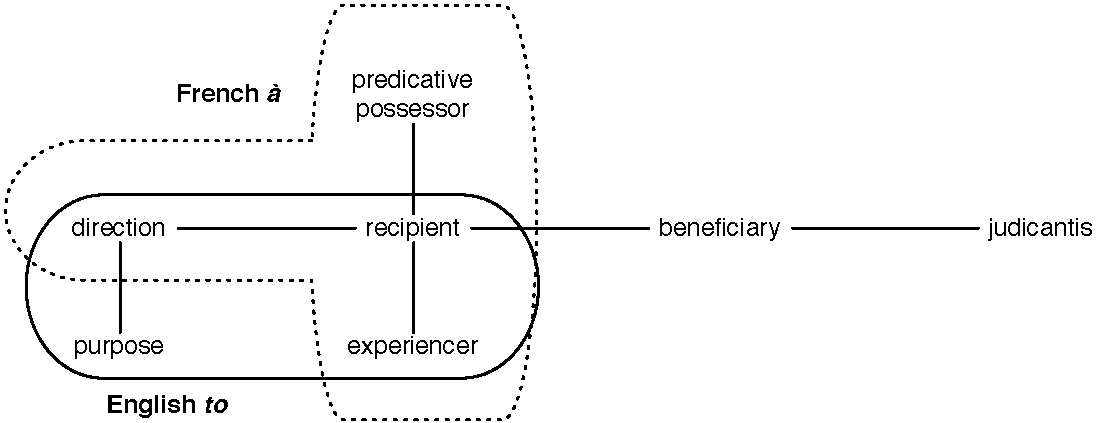
\includegraphics[width=\textwidth]{Chapter5/figs/semmap-to}}
  \caption[A semantic map\is{semantic maps} of dative\is{case!dative} functions for {\em to} \citep{haspelmath03geometry}]{This partial semantic map\is{semantic maps} compares the French\is{French} preposition\is{preposition} {\em \`{a}} to the English\is{English} preposition\is{preposition} {\em to} with respect to which typical dative\is{case!dative} functions they cover. Non-dative\is{case!dative} functions are ignored in this map \citep[adapted from][figures 8.1 and 8.2, p. 213 and 215]{haspelmath03geometry}.}
   \label{f:semmap-to}
\end{figure}

Semantic maps depend crucially on cross-linguistic research. For example, a node in the network is only added if at least one language is found which makes the distinction. Haspelmath gives the example of direction\is{semantic role!direction} versus recipient\is{semantic role!recipient} (p. 217). Based on English\is{English} and French\is{French}, which use one preposition\is{preposition} for
both functions, this distinction could not be made. However, German\is{German} uses {\em zu} or {\em nach} for direction\is{semantic role!direction}, whereas it uses the dative\is{case!dative} case for recipient\is{semantic role!recipient}. A large sample set of languages is therefore needed to uncover all the uses of a gram.

Another important aspect of semantic map\is{semantic maps}s is the connection between nodes in the network. The map must represent these nodes in a contiguous area on the map. Haspelmath writes that based on the English\is{English} preposition\is{preposition} {\em to}, for example, the following three orders could be possible for purpose\is{semantic role!purpose}, direction\is{semantic role!direction} and recipient\is{semantic role!recipient} (p. 217, example 4):

\eal
\ex[]{purpose\is{semantic role!purpose} -- direction\is{semantic role!direction} -- recipient\is{semantic role!recipient}}
\ex[]{direction\is{semantic role!direction} -- purpose\is{semantic role!purpose} -- recipient\is{semantic role!recipient}}
\ex[]{ direction\is{semantic role!direction} -- recipient\is{semantic role!recipient} -- purpose\is{semantic role!purpose}}
\zl

Again, data from other languages are taken into account for choosing which option can be eliminated. Since the French\is{French} preposition\is{preposition} {\em \`{a}} cannot be used for marking purpose\is{semantic role!purpose}, option (b) cannot represent a contiguous space in the network. The German\is{German} preposition\is{preposition} {\em zu} eliminates option (c) because it can express purpose\is{semantic role!purpose} and direction\is{semantic role!direction}, but not recipient\is{semantic role!recipient}. The direct connections between functions on the semantic map\is{semantic maps} are important because they are hypothesized to be universal:

\begin{quote}
Semantic maps not only provide an easy way of formulating and visualizing differences and similarities between individual languages, but they can also be seen as a powerful tool for discovering universal semantic features that characterize the human language capacity. Once a semantic map\is{semantic maps} has been tested on a sufficiently large number of languages [...] from different parts of the world, we can be reasonably confident that it will indeed turn out to be universal. \citep[p. 232]{haspelmath03geometry} 
\end{quote}

This view is shared by many other linguists, among whom Bill Croft. Croft's {\em Semantic Map Connectivity Hypothesis\is{Semantic Map Connectivity Hypothesis}} \citep[p. 96]{croft01radical} states that the functions of a particular construction will always cover functions that are connected regions in {\em conceptual space\is{conceptual space}}. In other words, grammatical categories are language-particular, but they are based on a universal conceptual/semantic space.

The universality of semantic map\is{semantic maps}s is however an issue of debate. For example, \citet{cysouw08building} reports on his attempts at making a satisfying map for person marking. He concludes that there is no single `universal' semantic map\is{semantic maps}. Instead, different semantic map\is{semantic maps}s are possible depending on the level and granularity of the analysis. Cysouw therefore calls for using semantic map\is{semantic maps}s as a tool for modeling attested linguistic variety and as a way to predict {\em probable} languages rather than {\em possible} languages by weighting the function nodes in the network depending on the number of attested cases.

Cysouw thus points to a serious problem of the semantic map\is{semantic maps} hypothesis: what grain-size is acceptab\is{acceptability}le for making semantic map\is{semantic maps}s? For example, \citet{haspelmath03geometry} uses functions such as `recipient\is{semantic role!recipient}' and `beneficiary\is{semantic role!beneficiary}' as primitive categories for his analysis. However, these functions are language-specific and no grammatical category has been demonstrated to cover all possible instantiations of such a function. Instead, languages tend to have many exceptions, irregularities or a redundant overlap in categories that mark that function. For example, `recipient\is{semantic role!recipient}' and `beneficiary\is{semantic role!beneficiary}' not only occur with the preposition\is{preposition}s {\em to} and {\em for} respectively, they can also take the first object\is{syntactic role!object} position in the English\is{English} ditransitive\is{ditransitive clause}.

The universality hypothesis therefore faces a problem of circularity. On the one hand, semantic map\is{semantic maps}s are hypothesized to represent universal conceptual space\is{conceptual space}; on the other hand, that conceptual space\is{conceptual space} is based on an analysis which ignores language-internal differences and irregularities, and the languages that do not mark any differences are still assumed to have the same underlying functions.

Artificial language evolution\is{artificial language evolution} could demonstrate an alternative hypothesis to explain the universal tendencies in grammatical marking. In problem-solving\is{problem-solving} models such as this book, grammatical evolution\is{evolution!cultural evolution} is a consequence of distributed processes whereby language users shape and reshape their language. The main challenge is therefore to find out what these processes are and under what circumstances they could create the kind of semantic map\is{semantic maps}s that are observed for human languages. The hypothesis is that these processes suffice for the emergence\is{emergence} of semantic map\is{semantic maps}s and that conceptual space\is{conceptual space} is dynamically configured in co-evolution with grammar. Semantic maps of different languages will naturally show similarities and differences depending on whether they followed the same evolutionary pathways or not.
\\
\\
\noindent{\bfseries Prior work on concept\is{concept formation} emergence.} As mentioned in section \ref{s:history-of-research}, prior work in the field has already demonstrated how a population\is{speech population} of agents could self-organiz\is{self-organization}e a shared ontology through communicative interactions. \citet{steels97constructing} reports the first experiments in which conceptualization\is{conceptualization} and lexicon\is{lexicon} emergence are coupled to each other. In the experiment, a population\is{speech population} of artificial agents take turns in playing `guessing game\is{language game!guessing game}s': the speaker chooses one of the objects in the context to talk about and wants to draw the hearer's attention to it by saying a word. The game is a success if the hearer points to the correct object. If the game fails, the speaker will point to the intended topic and the hearer tries to guess what the speaker might have meant with his word. The agents start without any language and even without an ontology. Instead, they are equipped with several sensory channels for perceiving the objects in their environment.

At the start of a game, two agents are randomly chosen from the population\is{speech population} to act as a speaker and as a hearer. The speaker chooses an object from the context to talk about and needs to conceptualize a meaning which discriminates the topic from the other objects in the context. For example, if the topic is a green ball and there are also three red balls in the context, then the topic's colour\is{colour} would be a good discriminating feature. At the beginning of the experiment, the agents have no concepts yet so the speaker has to create a new one. He will do so by taking the minimal set of features that can discriminate the topic from the other objects. The speaker will then invent a new word for this concept\is{concept formation} or meaning and transmit it to the hearer.

The hearer will in turn experience a communicative problem: He does not know the word that was used by the speaker. The game thus fails, but the speaker points to the intended object. The hearer then tries to retrieve the intended meaning through the same discrimination game\is{discrimination game}. Often there are many different sets of discriminating features possible, but if the agents play a sufficient amount of language game\is{language game}s with each other, they come to an agreement on what the form-meaning pairs are in their language and thus also reach a shared conceptual space\is{conceptual space}. Similar experiments have been successfully performed in the domains of colour\is{colour} terms \citep{steels05coordinating} and spatial\is{spatial language} language \citep{steels08perspective-alignment}, and they have been scaled up to large meaning spaces \citep{wellens08coping}.
\begin{figure}[t]
\centerline{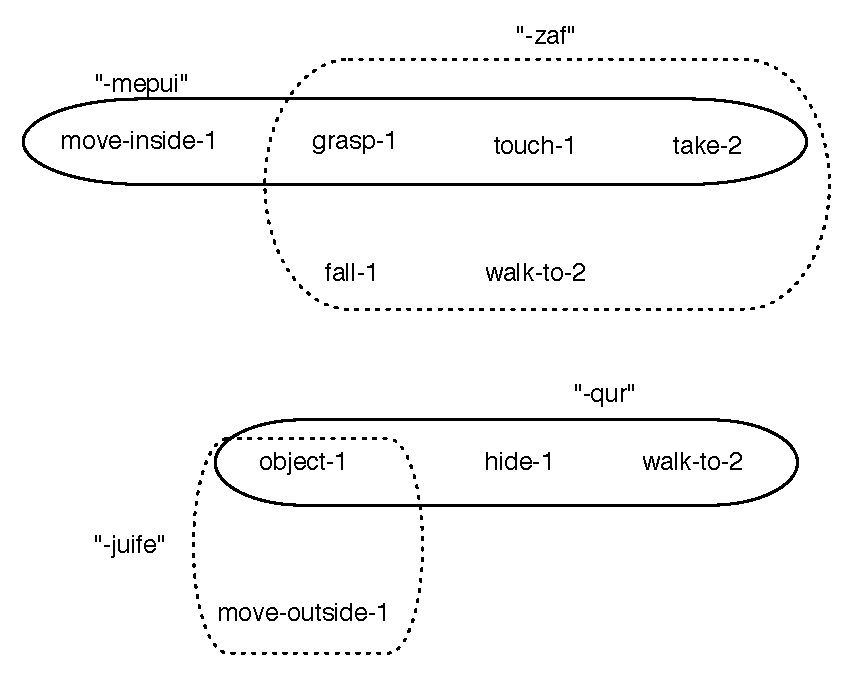
\includegraphics[scale=0.7]{Chapter5/figs/sem-map1}}
  \caption[Two `semantic map\is{semantic maps}s' from the experiments]{This diagram compares two different artificial grammars with respect to two categories in each of them. The languages were formed using the final set-up of experiment 3 (section \ref{s:pattern-exp-3}). Even though the agents did not have a continuous conceptual space\is{conceptual space} in advance, it is nevertheless possible to draw a primitive semantic map\is{semantic maps} afterwards.}
   \label{f:semmap-1}
\end{figure}
\\
\\
\noindent{\bfseries The contribution of this book.} All of the above experiments confirm that communicative success\is{communicative success} can be a driving force for constructing an ontology of meaningful distinctions and that language can be used as a way to agree on a shared ontology among a population\is{speech population} of autonomous embodied artificial agents. These experiments, however, have only focused on concept-and-lexicon\is{lexicon} emergence so far, and the systematic relations between words have not been investigated yet. The experiments in this book, however, have polysemous semantic role\is{semantic role}s so they form an ideal starting point for testing the alternative hypothesis.

Figure \ref{f:semmap-1} illustrates how analog\is{analogy}ical reasoning can be responsible for constructing coherent classes of semantic role\is{semantic role}s. The diagrams shows two semantic map\is{semantic maps}s for two languages that were formed in the last set-up of experiment 3 as described in section \ref{s:pattern-exp-3} (multi-level selection\is{selection}\is{multi-level selection} with memory decay\is{memory decay} and pattern formation\is{pattern formation}\is{formation}). Both diagrams show that it is possible to draw a primitive semantic map\is{semantic maps} which compares the semantic role\is{semantic role}s of both languages. For example, in one language the marker\is{case!case marking} {\em -mepui} can be used for covering four participant role\is{participant role}s. Three of them (grasp-1, touch-1 and take-2) overlap with a semantic role\is{semantic role} of a different language. A similar observation counts for the two semantic role\is{semantic role}s in the second semantic map\is{semantic maps}.

A comparison of the formed artificial languages suggests that grammaticalization\is{grammaticalization} processes can be visualized as a movement or change in connected regions of a continuous domain as a side-effect of analog\is{analogy}ical reasoning: exten\is{extension}sion of a category happens when new situations are encountered which are closely related to the existing categories. This shows that semantic map\is{semantic maps}s could in principle be the result of dynamic processes involving analog\is{analogy}y rather than starting from universal conceptual space\is{conceptual space}.

The alternative proposed here needs further investigation and essentially requires a significant scale-up in terms of the meaning space and world environment as well as the conceptualization\is{conceptualization} capabilities of the agents. The present results are however encouraging and the proposed alternative has the advantage that it is more adaptive and open-ended to a changing environment: a universal conceptual space\is{conceptual space} would still require some mechanism of mapping culture-specific developments (such as buying and selling, driving cars, and steering airplanes) onto a prewired structure. If the alternative hypothesis is followed, semantic map\is{semantic maps}s would thus not point to a universal map of human cognition but rather to recurrent patterns in human experience and preferred developmental pathways followed by dynamic categorization mechanisms.

\subsection{Thematic hierarchies in case systems\is{case!case system}}
\label{s:comp-thematic}

\begin{figure}[t]
\centerline{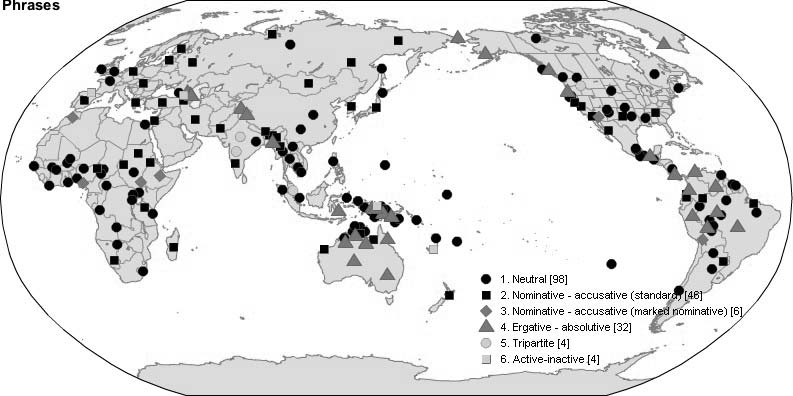
\includegraphics[width=\textwidth]{Chapter5/figs/wals.jpg}}
  \caption[Alignment of case marking of full noun\is{noun} phrases \citep{comrie05wals}]{The alignment of case marking\is{case!case marking} of full noun\is{noun} phrases \citep[98]{comrie05wals}.}
   \label{f:wals}
\end{figure}

Many linguistic theories assume that argument linking is governed by a universal thematic hierarchy \citep[e.g.][]{dik97functional, fillmore68case, givon01syntax, jackendoff90semantic, keenan77noun}. However, empirical evidence shows that such hierarchies can offer tendencies at best, and that they cannot be considered as innate knowledge \citep{levin05argument}. Even for language-specific argument linking patterns, no satisfying hierarchy\is{hierarchy} has been found yet.

The question of how language systematicity\is{systematicity} can ever arise becomes a big issue if no universal hierarchy\is{hierarchy} can be found, especially if no Universal Grammar\is{Universal Grammar} is assumed. The map in Figure \ref{f:wals}, for example, shows the alignment of case marking\is{case!case marking} of full noun\is{noun} phrases across 190 languages. It clearly demonstrates strong systematicity\is{systematicity} in the marking of `core arguments' in these languages. \citet{comrie05wals} distinguishes five different systems\is{case!case system} (I count the two variants of nominative\is{case!nominative}-accusative\is{case!accusative} systems\is{case!case system} as one):

\begin{itemize}
\item Neutral: the subject\is{syntactic role!subject} of intransitive clause\is{intransitive clause}s (S) is marked in the same way as both the subject\is{syntactic role!subject} (A) and object\is{syntactic role!object} (P) of transitive clause\is{transitive clause}s. Example: Mandarin.
\item Nominative-accusative\is{case!accusative}: A and S are marked in the same way (nominative\is{case!nominative} marking). P is marked differently (accusative\is{case!accusative} marking). Example: Latvian\is{Latvian}.
\item Ergative-absolutive: S and P are marked in the same way (ergative marking), A is marked differently (absolutive marking). Example: Hunzib\is{Hunzib}.
\item Tripartite\is{case!tripartite case system}: S, A and P are all marked differently. Example: Hindi\is{Hindi}.
\item Active-inactive\is{active-stative languages}\is{construction!active construction}: There is a different marker\is{case!case marking} for an agentive S (aligning with A) and a patient\is{semantic role!patient}ive S (aligning with P). Example: Georgian\is{Georgian}. 
\end{itemize}

The answer for most linguists is again sought in universals. For example, \citet{croft98event} assumes a universal conceptual space\is{conceptual space} and universal linking rules for mapping arguments to core syntactic cases. The problem here is again that the proposals only work for analyses that do not go beyond the crude representation of case marking\is{case!case marking} systems\is{case!case system} as presented in Figure \ref{f:wals}. Closer studies show that the proposed systems\is{case!case system} are again only tendencies in each language and that there are lots of exceptions to the `default' alignment of case marking\is{case!case marking}. Also the typological variation\is{variation} across languages is greater than suggested by the traditional SAP-system of core arguments \citep{mithun05beyond}.
\\
\\
\noindent{\bfseries Analog\is{analogy}y, pattern formation\is{pattern formation}\is{formation} and multi-level selection\is{selection}\is{multi-level selection}.} In the case of thematic hier\is{thematic hierarchy}archies, a similar alternative can be devised based on the distributed processes whereby language users shape and reshape their language for communication. As I argued in Chapter \ref{c:base}, generaliz\is{generalization}ation of grammatical categories arises as a side-effect within inferential coding system\is{inferential coding system}s: language users want to increase their communicative success\is{communicative success} and when speakers have to solve a problem or innovat\is{innovation}e, they will try to do this in such a way that the intended communicative effect is still reached. By exploiting analog\is{analogy}y, the speaker can hook the new situation up to previous convention\is{convention}s which are probably known by the hearer as well. The hearer can then retrieve the intended meaning through the same mechanisms of analog\is{analogy}ical reasoning.

As categories get reuse\is{reuse}d more often, they increase their type frequency\is{type frequency}\is{frequency} and hence their productivity\is{productivity}. An additional factor that boosts the success of such a category is when it starts to form patterns or groups with other elements in the inventory. A multi-level selection\is{selection}\is{multi-level selection} alignment strateg\is{alignment strategy}y then assures that certain categories can also survive and reoccur in multiple levels of the linguistic network which again increases their frequency\is{frequency} and chances of survival. Multi-level selection\is{selection}\is{multi-level selection} could thus explain how different constructions align their categories with each other as demonstrated in the map in Figure \ref{f:wals}.

Preferences in argument linking, as predicted by thematic hier\is{thematic hierarchy}archies, could thus gradually emerge as a side-effect of these mechanisms: as certain categories become more and more dominant and productive, they can start to exten\is{extension}d their use across patterns and eventually evolve into prototypical subject\is{syntactic role!subject} and object\is{syntactic role!object} categories (as I also suggested in section \ref{s:stage4}). The many subregularities that are observed in languages are no problem in this model and are in fact predicted because everything has to emerge in a bottom-up fashion. Further experiments on the emergence of syntactic cases could thus be the starting point for modeling this alternative to thematic hier\is{thematic hierarchy}archies.

\subsection{A redundant approach to grammaticalization\is{grammaticalization}}
\label{s:actualization}

A third debate in which artificial language evolution\is{artificial language evolution} can offer novel insights is grammaticalization\is{grammaticalization} theory. As I already mentioned in section \ref{s:stage2}, one of the problems of grammaticalization\is{grammaticalization} is that linguists can usually only detect language change\is{language change} once the processes of grammaticalization\is{grammaticalization} have already taken place. It is therefore difficult to hypothesize what mechanisms should be proposed to explain such changes especially since the consequences of communicative interactions in larger population\is{speech population}s are often overlooked. Multi-agent simulations can thus demonstrate which mechanisms are better suited for dealing with innovat\is{innovation}ions, variation\is{variation}s, and propagat\is{propagation}ions of linguistic convention\is{convention}s.
\\
\\
\noindent{\bfseries Reanalysis and actualization\is{actualization}.} Diachronic reanalysis\is{reanalysis} has taken a foreground position in traditional grammaticalization\is{grammaticalization} theory. For example, \citet{hopper93grammaticalization} write: {\em ``Unquestionably, reanalysis\is{reanalysis} is the most important mechanism for grammaticalization\is{grammaticalization}''} (p. 32). Reanalysis is understood as a {\em ``change in the structure of an expression or class of expressions that does not involve any immediate or intrinsic modification of its surface manifestation}'' \citep[p. 59]{langacker77syntactic}. In other words, reanalysis\is{reanalysis} is not noticeable from the surface form but only has consequences for the grammar at a later stage. Many theories therefore posit another mechanism called `actualization' that maps out the consequences of reanalysis\is{reanalysis} \citep{timberlake77reanalysis}.

Reanalysis is typically illustrated by the grammaticalization\is{grammaticalization} of {\em be going to} into {\em gonna} \citep[p. 2--4]{hopper93grammaticalization}. In an older use of {\em be going to}, {\em to} was part of a purposive direction\is{semantic role!direction}al complement\is{complement} as in {\em I am going to marry Bill} meaning `I am going/travelling in order to marry Bill'. At a later stage, {\em to} is hypothesized to be reanalysed as belonging to {\em be going} instead of to the complement\is{complement}. In other words, rebracketing\is{rebracketing} of the structure has taken place from [[I] [am going] [to marry Bill]] to [[I] [am going to] [marry Bill]].

Reanalysis\is{reanalysis} has recently been challenged. \citet{haspelmath98does} writes that reanalysis\is{reanalysis} does not entail\is{entailment} a loss of autonomy which is typical for grammaticalization\is{grammaticalization} and that grammaticalization\is{grammaticalization} is (almost exclusively) unidirectional instead of bidirectional\is{bidirectionality} as predicted by reanalysis\is{reanalysis}. Haspelmath also rejects the combination of reanalysis\is{reanalysis} with actualization\is{actualization} which is often used as a way to assign gradualness to reanalysis\is{reanalysis} (p. 340--341). Actualization makes `reanalysis\is{reanalysis}' as a mechanism impossible to verify and it requires speakers to know at least two analyses of the same construction to account for both the old and the new behaviour. Actualization also does not explain how innovat\is{innovation}ions might propagat\is{propagation}e. Haspelmath's comparison of `grammaticalization' and `reanalysis\is{reanalysis}' is summarized in Table \ref{t:grammaticalization}.
\begin{table}
\centerline{\begin{tabular}{l l}
\hline
{\em Grammaticalization}\hspace{2,5cm} & {\em Reanalysis}
\\
\hline
loss of autonomy / substance & no loss of autonomy / substance
\\
gradual & abrupt
\\
unidirectional & bidirectional\is{bidirectionality}
\\
no ambiguity\is{ambiguity} & ambiguity\is{ambiguity} in the input structure
\\
due to language use & due to language acquisition\is{acquisition}
\\
\hline
\end{tabular}}
\caption[Major differences between grammaticalization\is{grammaticalization} and reanalysis \citep{haspelmath98does}]{This table shows the major differences between grammaticalization\is{grammaticalization} and reanalysis\is{reanalysis} \citep[p. 327, Table 1]{haspelmath98does}.}
\label{t:grammaticalization}
\end{table}

Despite the problems of reanalysis\is{reanalysis}, it seems hard to conceive an alternative process that could explain certain changes. Haspelmath suggests that formal theories should implement the gradience of membership of word classes in some way such as {\em ``V$_{1.0}$ for ordinary verb\is{verb}s, V$_{.7}$/P$_{.3}$ for preposition\is{preposition}-like verb\is{verb}s (e.g.} considering{\em) and so on''} (p. 330). Even though gradience is indeed an important matter, such a proposal cannot capture the fact that the old use of a linguistic item and its new function can co-exist\is{co-existence} for hundreds of years in a language. The alternative that I would propose is  redundancy\is{redundancy} and pattern formation\is{pattern formation}\is{formation} along the lines of my example for French\is{French} predicate negation\is{negation} in Chapter \ref{c:experiment1}. Applied to the example of {\em gonna}, this alternative would simply state that the frequent co-occur\is{co-occurrence}rence of the words {\em be going to} led to the creation of a pattern for optimizing linguistic processing. Once this pattern is created, it may start evolving on its own which allows it to gradually drift away from the original use of the words.
\\
\\
\noindent{\bfseries Example: the English\is{English} verb\is{verb}al gerund\is{gerund}.} To illustrate this alternative approach, I will briefly take a look at the English\is{English} verb\is{verb}al gerund\is{gerund} which historically developed from a deverbal nominalization\is{nominalization} and which later acquired more and more verb\is{verb}al properties. I will show examples of this development taken from \citet{fanego04reanalysis} and summarize how he describes this grammaticalization\is{grammaticalization} process in terms of `reanalysis\is{reanalysis}' and `actualization'. Next, I will argue for a simpler model based on  redundancy\is{redundancy} and pattern formation\is{pattern formation}\is{formation}.

The English\is{English} gerund\is{gerund} is a unique category in European languages in the sense that it is a third type of verb\is{verb}al complement\is{complement} besides  to-infinitive\is{to-infinitive}s (example \ref{e:gerund1}) and finite\is{finiteness} clauses (\ref{e:gerund2}). The present-day English\is{English} gerund\is{gerund} has the following verb\is{verb}al properties: it can take a direct object\is{syntactic role!object} (\ref{e:gerund3}), it can be modified by adverb\is{adverb}s (\ref{e:gerund4}), it can mark tense\is{tense}, aspect\is{aspect} and voice distinctions (\ref{e:gerund5}), it can be negated using the predicate negator {\em not} (\ref{e:gerund6}) and it can take a subject\is{syntactic role!subject} in a case other than the genitive\is{case!genitive} (\ref{e:gerund7}).

\ea
\label{e:gerund1}
I just called \emph{to say} `I love you'.
\item Just tell him \emph{we're not interested anymore}.
\label{e:gerund2}
\item By writing \emph{a book}, he managed to face all his inner demons.
\label{e:gerund3}
\item My \emph{quietly} leaving before anyone noticed.
\label{e:gerund4}
\item The necessity of \emph{being loved} is a driving force in our lives.
\label{e:gerund5}
\item My \emph{not} leaving the room caused a stir.
\label{e:gerund6}
\item We should prevent \emph{the treaty} taking effect.
\label{e:gerund7}
\z

Studies on the emergence\is{emergence} and evolution\is{evolution!cultural evolution} of the gerund\is{gerund} suggest that it developed from a deverbal nominalization\is{nominalization} construction, similar to phrases such as \emph{the writing of a book} \citep{tajima85syntactic}. This nominalization\is{nominalization} lacked the aforementioned verb\is{verb}al properties, which can be illustrated with a similar nominalization\is{nominalization} construction in Dutch\is{Dutch}: example \ref{e:gerund8} shows that the nominalized \emph{bewerking} `adaptation' cannot be complement\is{complement}ed by a direct object\is{syntactic role!object} (as is possible with the English\is{English} gerund\is{gerund}). Instead, it requires the genitival preposition\is{preposition} \emph{van} `of' (a). Example (c) shows that speakers of Dutch\is{Dutch} need to combine a preposition\is{preposition}al noun\is{noun} phrase with some kind of  to-infinitive\is{to-infinitive} to express one of the functions carried by the English\is{English} gerund\is{gerund}.

\eal
\label{e:gerund8}
\ex[ ]{ \gll de	bewerking 	van 		het 	stuk\\
the	adaptation	of	the	piece\\
\glt `the adaptation of the play'
}
\ex[ ]{ \gll *door 	bewerking 	het 	stuk\\
by	adaptation	 the	piece\\}
\ex[ ]{ \gll door	het	stuk	te	bewerken\\
by	the	piece	to	adapt\\
\glt `by adapting the play'}
\zl

From this kind of deverbal nominalization\is{nominalization}, the English\is{English} gerund\is{gerund} probably evolved according to the following steps (\citealp{tajima85syntactic}, summary and examples taken from \citealt{fanego04reanalysis}):

\begin{enumerate}
\item Around 1200, the deverbal nominalization\is{nominalization} \emph{-ing} began taking adverb\is{adverb}ial modifiers of all kinds:

\ea
Of \th i comyng at domesday\\
{\em `Of your coming \emph{at doomsday}.'}
\z

\item The first examples with direct object\is{syntactic role!object}s have been attested around 1300.

\ea
yn feblyng \th e body with moche fastyng
\\ {\em `in weakening the body by too much abstinence'}
\z

\item In the Early Modern English\is{English} period, other verb\is{verb}al features are increasingly found, such as distinctions of voice and tense\is{tense}. From Late Modern English\is{English} on, gerund\is{gerund}s also start to take subject\is{syntactic role!subject}s:

\ea 
he was war of hem comyng and of here malice \\
{\em `he was informed of them coming and of their wickedness'}
\z
\end{enumerate}

\citet{fanego04reanalysis} argues that these changes are best understood as reanalysis\is{reanalysis} of a nominal structure to a (more) verb\is{verb}al one (p. 26). This requires the speaker's ability to recognize multiple structural analyses since the `old' and the `new' use co-exist\is{co-existence}ed for a long time. The following examples show how the nominal analysis and the more verb\is{verb}al structure could be used together around 1300, whereas nowadays the nominal structure is unacceptab\is{acceptability}le unless there is a determiner\is{determiner}:

\ea
\label{e:gerund-last}
Sain Jon was ... bisi In ordaining of priestes, and clerkers, And in planning kirc werkes.\\
{\em `Saint John was ... busy ordaining priests and clerics, and in planning church works.'}

\item the ordaining of priests / the planning of works
\item ordaining priests / planning works
\item *ordaining of priests / *planning of works
\z

In order to account for the gradualness of the change, Fanego suggests a reanalysis-plus-actualization model. He acknowledges \citet{haspelmath98does}'s criticism on this model that it is still not gradual enough and he proposes that the gerund\is{gerund} should be regarded as a hybrid category which is partly noun\is{noun} and partly verb\is{verb}. To summarize, Fanego suggests that the development of the various uses of the English\is{English} gerund\is{gerund} involved (a) reanalysis\is{reanalysis} and (b) actualization\is{actualization} using Haspelmath's proposal for gradient categories. 
\\
\\
\noindent{\bfseries Problems with Fanego's account.} Fanego's analysis of the development of English\is{English} requires complex cognitive operations from the part of the speaker that do not seem entirely justified. First of all, in order to reconcile reanalysis\is{reanalysis} with the data, he needs to call on the process of actualization\is{actualization}. However, as \citet{haspelmath98does} already noted, actualization\is{actualization} {\em ``waters down the notion of reanalysis\is{reanalysis}, because it allows one to posit non-manifested reanalysis\is{reanalysis} as one pleases''} (p. 341). It also seems contradictory to propose reanalysis\is{reanalysis}, which is essentially an abrupt and discrete process, together with Haspelmath's gradient categories. Mechanisms such as semantic bleaching\is{semantic bleaching}, analog\is{analogy}y and exten\is{extension}sion could explain a gradual shift from a nominal category to a more verb\is{verb}-like category just as well without evoking reanalysis\is{reanalysis}.

A second problem has to do with the idea of a gradient category, that is, analyzing the gerund\is{gerund} as some hybrid category which is let's say 20\% nominal and 80\% verb\is{verb}al. This kind of analysis treats the Gerund as a single category in the grammar whereas Fanego himself distinguishes at least three different types existing today, each with their own particular syntactic behaviours:

\begin{itemize}
\item Type 1: gerund\is{gerund}s lacking determiner\is{determiner}s (e.g. {\em by writing it})
\item Type 2: gerund\is{gerund}s taking determiner\is{determiner}s (e.g. {\em the writing of the letter})
\item Type 3: verb\is{verb}al gerund\is{gerund} (e.g. {\em the people living in this town})
\end{itemize}

\noindent{\bfseries A model based on  redundancy\is{redundancy}.} Reanalysis is a mechanism which is based on mismatches in learning. In the case of the English\is{English} gerund\is{gerund}, Fanego writes that the first gerund\is{gerund}s to take verb\is{verb}al traits were the ones occurring in constructions without determiner\is{determiner}s (p. 19--20). However, the lack of determiner\is{determiner}s is in itself not necessarily a reason for reanalyzing a grammatical structure, especially since determiner\is{determiner}s were not at all obligatory in many noun\is{noun} phrases in Old and Middle English\is{English} \citep[p. 172--174]{traugott92syntax}. One can therefore reverse the question and ask why some uses of the gerund\is{gerund} resisted the spread of determiner\is{determiner}s. In other words: is there a {\em functional} explanation for the development of the gerund\is{gerund}?

A first step in the alternative hypothesis is to accept  redundancy\is{redundancy}: language users store many instances in memory so rather than looking for a single category which leads to multiple structural analyses, speakers are assumed to store many instances in memory. Actual change in the system only takes place if one of these redundant instances gets exten\is{extension}ded. No layering\is{synchron\is{synchronic}ic layering} or complex mechanisms for disambiguity\is{ambiguity} are needed since there are still enough instances left that cover the older use of a particular form. Redundancy thus requires a far more simple cognitive model than the reanalysis-and-actualization approach and treats each use of the gerund\is{gerund} as a construction in its own right.

Instead of reanalysis\is{reanalysis} and mismatches in learning, the alternative hypothesis assumes that some patterns or instances exten\is{extension}d their usage for a communicative reason. Fanego lists several possible sources (p. 11--17): first of all, the {\em-ing}-form of nominalization\is{nominalization}s was in competit\is{competition}ion with the Old English\is{English} present participle {\em -ende} (which still exists in Dutch\is{Dutch}, for example). {\em -ing} became dominant by the fifteenth century and thus increased its frequency\is{frequency}. Along with this competit\is{competition}ion, the productivity\is{productivity} of {\em -ing} also increased from a limited number of verb\is{verb}s to an almost fully productive schema. A third possible source could be the fact that the English\is{English}  to-infinitive\is{to-infinitive} has resisted the combinations with other preposition\is{preposition}s than {\em to} and {\em for to}. This created a gap in the usage of the infinitive which could be filled by the gerund\is{gerund} (or conversely, the expansion of the gerund\is{gerund} prevented the infinitive from filling this gap itself). Other sources are influences from French\is{French} and the co-occur\is{co-occurrence}rence of the gerund\is{gerund} with a genitive\is{case!genitive} phrase.

The point here is not to find {\em the} source for the development of the English\is{English} gerund\is{gerund} but rather to illustrate that many possible sources can be identified and that they all probably played some role. It is therefore fruitful to see language as a selection\is{selection}ist system in which all linguistic items compete for a place in the inventory. Due to multi-level selection\is{selection}\is{multi-level selection}, categories can become more dominant across patterns which is what seemed to have happened with the gerund\is{gerund}: it increased its productivity\is{productivity}, won the competit\is{competition}ion against {\em -ende} for marking participles and hence became more frequent and successful.

\citet{haspelmath98does} also criticized reanalysis\is{reanalysis} for failing to explain the strong unidirectional tendency of grammaticalization\is{grammaticalization}. In a system of multi-level selection\is{selection}\is{multi-level selection}, this could be explained due to the fact that once linguistic items become part of larger patterns or occur in multiple constructions, they are no longer fully independent of those constructions. The benefit of belonging to larger groups is that each item's individual survival chances increase, but the possible downside could be that the original use becomes structurally ambiguous or that it loses its distinctiveness. This would weaken its position and leaves the possibility for other items to conquer its space. In other words, there are always two factors influencing survival of a linguistic item: frequency\is{frequency} and function.
\\
\\
\noindent{\bfseries Back to the computational model.} The above analysis is only an illustration of how computational modeling could inspire linguists to come up with alternative hypotheses. The grammaticalization\is{grammaticalization} model of  redundancy\is{redundancy} that I presented here mainly comes from the observation that variation\is{variation} in a population\is{speech population} is an extremely challenging problem and that it is very difficult for a population\is{speech population} to reach a shared and coherent language without losing generaliz\is{generalization}ation accuracy. Moreover, the design stance\is{design stance} can offer mechanisms and operationalizations that are simpler than the processes that are often proposed in verb\is{verb}al theories.

That said, the experiments presented in this book have not yet offered any proof that an analysis such as the one proposed here can actually work. However, they did show that a redundant and bottom-up approach {\em can} deal with high degrees of uncertainty in the development of a grammar whereas no such model exists (yet) for reanalysis\is{reanalysis}. The comparison between the Iterated Learning Model\is{Iterated Learning Model (ILM)} (which essentially relies on reanalysis\is{reanalysis}) and this book has shown that a usage-based approach\is{usage-based model} performs significantly better than a reanalysis\is{reanalysis} model. This does not mean that reanalysis\is{reanalysis} does not exist or that it cannot be operationalized, but it poses some serious challenges to the effectiveness and explanatory power of the mechanism.
